\documentclass[a4paper, 10pt]{article}
\usepackage{amsmath}
\usepackage{amsthm}
\usepackage{amsfonts}
\usepackage{amssymb}
\usepackage[italian]{babel}
\usepackage[utf8x]{inputenc}
\usepackage{mathtools}
\usepackage{listings}
\usepackage{amsfonts, mathtools, placeins, floatflt, xfrac, multirow, indentfirst, fancyhdr,
            amssymb, latexsym, amsthm, eucal, float, tabularx, mdframed, bigdelim, blkarray,
            relsize, lettrine, xcolor, tikz, caption, geometry, perpage}
\usepackage[tiny]{titlesec}
\usepackage{lmodern}
\usepackage{tikz}
\usepackage{subcaption}
\usepackage[object=vectorian]{pgfornament}
\usetikzlibrary{calc}

\newcommand{\sectionline}[2]{%
  \nointerlineskip \vspace{.5\baselineskip}\hspace{\fill}
  {\color{#1}
    \resizebox{0.5\linewidth}{2ex}
    {{%
    {\begin{tikzpicture}
    \node  (C) at (0,0) {};
    \node (D) at (9,0) {};
    \path (C) to [ornament=#2] (D);
    \end{tikzpicture}}}}}%
    \hspace{\fill}
    \par\nointerlineskip \vspace{.5\baselineskip}
  }



 \makeatletter

\def\vhrulefill#1{\leavevmode\leaders\hrule\@height#1\hfill \kern\z@}

\makeatother

\newcommand{\persendchap}{

	\center 	{\vhrulefill{0.9pt} \pgfornament[scale = 0.50, symmetry=v, ydelta = -0.5pt]{11} FINE CAPITOLO \pgfornament[scale = 0.50, ydelta=-0.5pt]{11} \vhrulefill{0.9pt} }
	\flushleft

}

%\renewcommand\thechapter{\arabic{chapter}}
\definecolor{mygreen}{RGB}{28,172,0} 
\definecolor{mylilas}{RGB}{170,55,241}

\lstloadlanguages{Matlab, Fortran}
 \lstset{
         basicstyle=\footnotesize\ttfamily, 
         numbers=left,              
         morekeywords={matlab2tikz},
         numberstyle=\tiny,        
         numbersep=5pt,           
         tabsize=2,                 
         extendedchars=true,        
         breaklines=true,           
         keywordstyle=\color{blue},
            frame=b,
         showspaces=false,          
         showtabs=false,            
         xleftmargin=17pt,
         framexleftmargin=17pt,
         framexrightmargin=5pt,
         framexbottommargin=4pt,
         showstringspaces=false     
              morekeywords=[2]{1}, keywordstyle=[2]{\color{black}},
    identifierstyle=\color{black},%
    stringstyle=\color{mylilas},
    commentstyle=\color{mygreen},%
    showstringspaces=false,
 }


\usepackage{caption}
\DeclareCaptionFont{white}{\color{white}}
\DeclareCaptionFormat{listing}{\colorbox[cmyk]{0.43, 0.35, 0.35,0.01}{\parbox{\textwidth}{\hspace{15pt}#1#2#3}}}
\captionsetup[lstlisting]{format=listing,labelfont=white,textfont=white, singlelinecheck=false, margin=0pt, font={bf,footnotesize}}
\newtheorem{mydef}{Definizione}
\begin{document}
\renewcommand{\lstlistingname}{Codice}

\begin{titlepage}
	\begin{center}
 		\includegraphics[scale=0.30]{logo/LOGO}\\
				
		\vspace{1.0cm}
		\Huge  Relazione \\ \vspace{0.3cm} di\\ \vspace{0.3cm} Metodi Numerici per la Grafica \\
		\vspace{1.5 cm}
		\Large  Di \vspace{0.2cm} \\ Federico Schipani 

		 \vfill                   
      A.A. 2017-2018
      \vspace{1cm}

    %  \begin{tikzpicture}
    %\node  (C) at (0,0) {};
    %\node (D) at (9,0) {};
    %\path (C) to [ornament=70] (D);
    %\end{tikzpicture}
      \vfill   
	\end{center}
\end{titlepage}

\tableofcontents
\newpage
%\vspace{30mm}

%\begin{tikzpicture}[every node/.style={inner sep=0pt}]
%\node[text width=8cm,align=center](Text){%
%
%
%La matematica è una delle manifestazioni più significative dell'amore per la sapienza. Come tale è caratterizzata da un lato da una grande libertà, 
%dall'altro dall'intuizione che il mondo è fatto di cose visibili e invisibili e la matematica ha forse una capacità, unica fra le altre scienze, 
%di passare dall'osservazione delle cose visibili all'immaginazione delle cose invisibili. Questo forse è il segreto della forza della matematica.
%
%
%\bigskip
%
%\vspace{24pt}
%  Ennio De Giorgi
%} ;
%\node[shift={(-1cm,1cm)},anchor=north west](CNW)  at (Text.north west)
%               {\pgfornament[width=2cm]{61}};
%\node[shift={(1cm,1cm)},anchor=north east](CNE)   at (Text.north east)
%               {\pgfornament[width=2cm,symmetry=v]{61}};
%\node[shift={(-1cm,-1cm)},anchor=south west](CSW) at (Text.south west)
%               {\pgfornament[width=2cm,symmetry=h]{61}};
%\node[shift={(1cm,-1cm)},anchor=south east](CSE)  at (Text.south east)
%               {\pgfornament[width=2cm,symmetry=c]{61}};
%\pgfornamenthline{CNW}{CNE}{north}{87}
%\pgfornamenthline{CSW}{CSE}{south}{87}
%\pgfornamentvline{CNW}{CSW}{west}{87}
%\pgfornamentvline{CNE}{CSE}{east}{87}
%\end{tikzpicture}
%
%
%\titleformat{\chapter}[display]
%  {\normalfont\huge\bfseries\raggedleft}
%  {\begin{tikzpicture}
%  \node[text width=3cm,align=center] (chapnum)
%    {\fontsize{100}{130}\color{gray}\selectfont\thechapter};%
%  \node[shift={(-1cm,1cm)},anchor=north west](CNW)
%    at (chapnum.north west) {\pgfornament[width=1.75cm]{61}};
%  \node[shift={(1cm,1cm)},anchor=north east](CNE)
%    at (chapnum.north east) {\pgfornament[width=1.75cm,symmetry=v]{61}};
%  \node[shift={(-1cm,-1cm)},anchor=south west](CSW)
%    at (chapnum.south west) {\pgfornament[width=1.75cm,symmetry=h]{61}};
%  \node[shift={(1cm,-1cm)},anchor=south east](CSE)
%    at (chapnum.south east) {\pgfornament[width=1.75cm,symmetry=c]{61}};
%  \end{tikzpicture}
%  }
%  {20pt}
%  {\Huge}

\section{La Base delle B-Spline}

Dato un vettore esteso dei nodi
$$ \mathbf{t} =  \left\{ \underbrace{t_{0}, \dots, t_{k-2}}_{k-1}, \underbrace{t_{k-1}, \dots, t_{n+1}}_{\tau_0, \tau_1, \dots, \tau_L}, \underbrace{t_{n+2}, \dots, t_{n+k}}_{k-1} \right\} $$
con
$$\mathbf{t_0} \leq t_1 \leq \dots t_{k+1} < t_k \dots < t_{n+1} \leq t_{n+2} \leq \dots \leq t_{n+k}$$
possiamo definire la base delle B-Spline su nodi semplici tramite la relazione ricorrente di \textit{Cox - Boor}.
\begin{mydef}
  Le B-Spline di ordine $1$, oppure grado $0$ sono definite come:
$$N_{i, 1}(t) = \begin{cases} 1, & \text{se } t\in[t_i, t_{i+1}] i = 0, \dots, n+k-1 \\ 0, & \text{altrimenti} \end{cases}$$
  Altrimenti le B-Spline di ordine $r \leq k$ sono definite ricorsivamente, per $r > 1$, come:
  $$N_{i, r}(t) = \omega_{i,r}(t)N_{i, r-1}(t) + [1-\omega_{i+1, r}(t)]N_{i+1, r-1}$$
  dove
$$\omega_{i,r}(t) = \begin{cases} \frac{t-t_i}{t_{i+r-1}-t_i}, & \text{se } t<t_{i+r-1} \\ 0, & \text{altrimenti} \end{cases}$$
\end{mydef}
Le B-Spline possono anche essere definite su una partizione nodale la cui molteplicità $m_i$ di un generico nodo $\tau_i$ è più alta di $1$,
quindi su nodi multipli. In questo caso il vettore esteso dei nodi diventa:
$$ \mathbf{t} =  \left\{ \underbrace{t_{0}, \dots, t_{k-2}}_{k-1}, \underbrace{t_{k-1}, \dots, t_{n+1}}_{\tau_0, \tau_1, \dots, \tau_1 \dots, \tau_L}, \underbrace{t_{n+2}, \dots, t_{n+k}}_{k-1} \right\} $$
con $\tau_i$ ripetuto a seconda della sua molteplicità $m_i$ con $i = 1, \dots, L-1$ in $\mathbf{t}$, e
$$\mathbf{t_0} \leq t_1 \leq \dots t_{k+1} \leq  t_k \dots \leq  t_{n+1} \leq t_{n+2} \leq \dots \leq t_{n+k}$$
La definizione della base delle B-Spline di \textit{Cox - De Boor} non cambia, ma bisogna stare attenti in quanto 
$\omega_{i,r}(t)$ può diventare nullo per qualche valore $r$  a causa dei nodi multipli.
In Codice \ref{code:functioncoxdeboor} sono mostrate le due funzioni che calcolano le basi di \textit{Cox - De Boor}, realizzate senza l'utilizzo delle funzioni del 
\textit{Curve Fitting Toolbox}.
\lstinputlisting[label=code:functioncoxdeboor, firstline=17, language=Matlab, caption = Calcolo delle basi di Cox De Boor]{code/cox_de_boor_basis.m}
La funzione \texttt{calc\_omega} di Codice~\ref{code:functioncoxdeboor} è di facile comprensione. Dati in input
l'indice $i$, l'ordine $r$, il punto in cui si vuole calcolare la spline $t\_star$ ed il vettore esteso dei nodi $\mathbf{t}$ si occupa di calcolare i valori $\omega_{i, r}(t)$.
%TODO: CORREGGERE PARENTESI TONDE IN TEXTTT
Il controllo iniziale \texttt{t\( i \) == t\( i+r-1 \)} serve a gestire il caso di nodi multipli. In questa particolare condizione possiamo trovarci a gestire casi in cui il denominatore di $\frac{t - t_i}{t_{i+1-r}-t_i}$ è uguale a $0$; quindi
$\omega_{i,r}(t)$ dev'essere posto a $0$. 
La seconda funzione in Codice~\ref{code:functioncoxdeboor} è \texttt{de\_boor\_basis} che effettua il calcolo delle basi delle B-Spline. 
La condizione booleana a riga 16, 17 e 18 serve a verificare che, nel caso 
in cui l'ordine della spline sia $1$, ci si trovi all'interno dell'intervallo $[t_i, t_{i+1} )$. Bisogna però fare attenzione al caso in cui 
il punto $t = t\_star$ di $N_{i, k}(t)$ si trovi nell'ultimo intervallo. Questo ha reso necessario introdurre un ulteriore controllo per fare in modo che venga 
preso in considerazione anche l'ultimo valore dell'ultimo intervallo.
\subsection{Esempi di basi}
L'esempio più immediato di base è quello dove il vettore esteso dei nodi è uniforme, in questo caso abbiamo preso $\mathbf{t} = [0, 1, 2, 3, 4, 5, 6, 7, 8, 9]$ e $k = 5$, otterremo quindi $5$
funzioni di base visualizzate in Figura~\ref{fig:first_basis}.
\begin{figure}[]
  \centering
  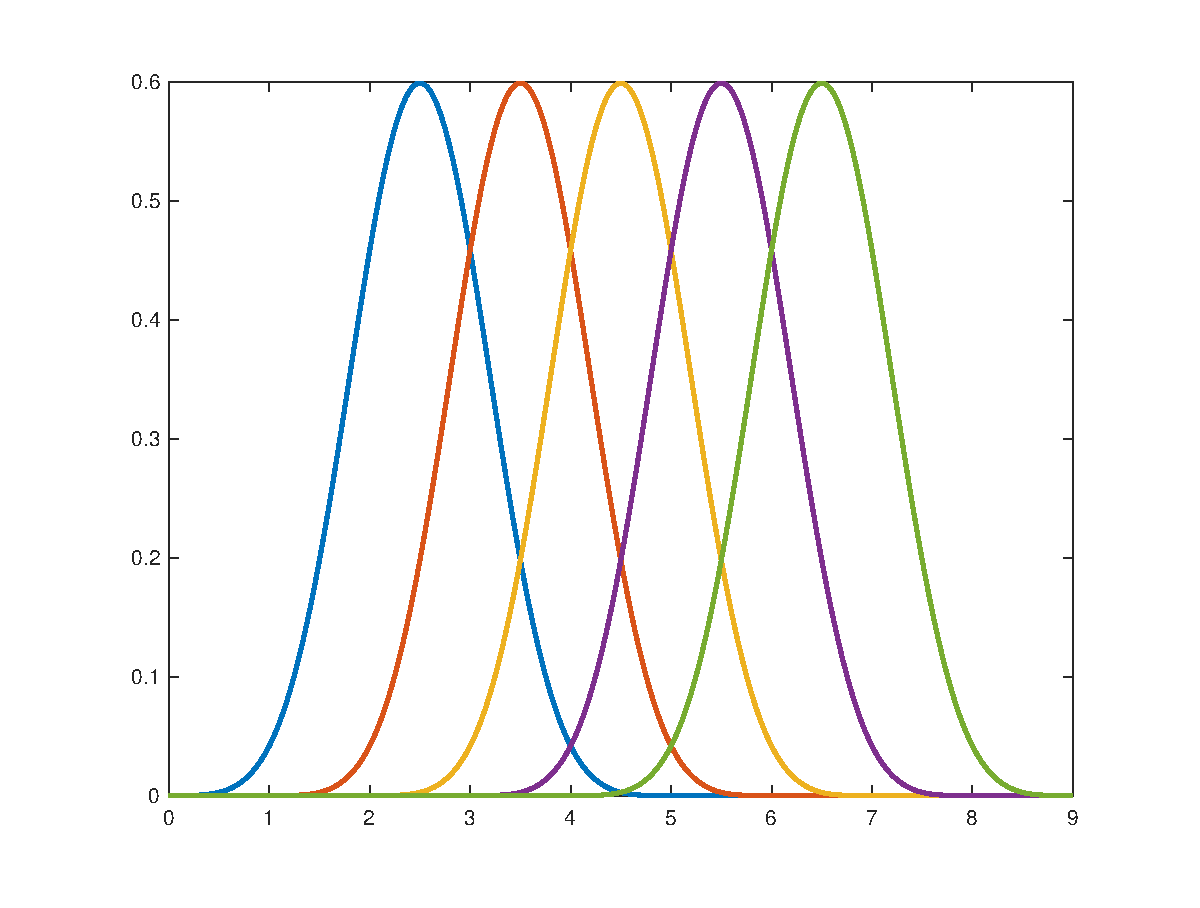
\includegraphics[width=0.75\textwidth]{figure/uniform_not_multiple_basis.eps}
  \caption{Base con $\mathbf{t} = [0, 1, 2, 3, 4, 5, 6, 7, 8, 9]$ e $k = 5$}
  \label{fig:first_basis}
\end{figure} 

Cambiando il vettore esteso dei nodi $\mathbf{t}$ otteniamo basi per le B-Spline con regolarità diversa.
In Figura~\ref{fig:animals} viene mostrato cosa succede tenendo fissato il numero di nodi e l'ordine e aumentato la molteplicità del nodo $4$.

\begin{figure}[]
  \centering
  \begin{subfigure}[b]{0.3\textwidth}
    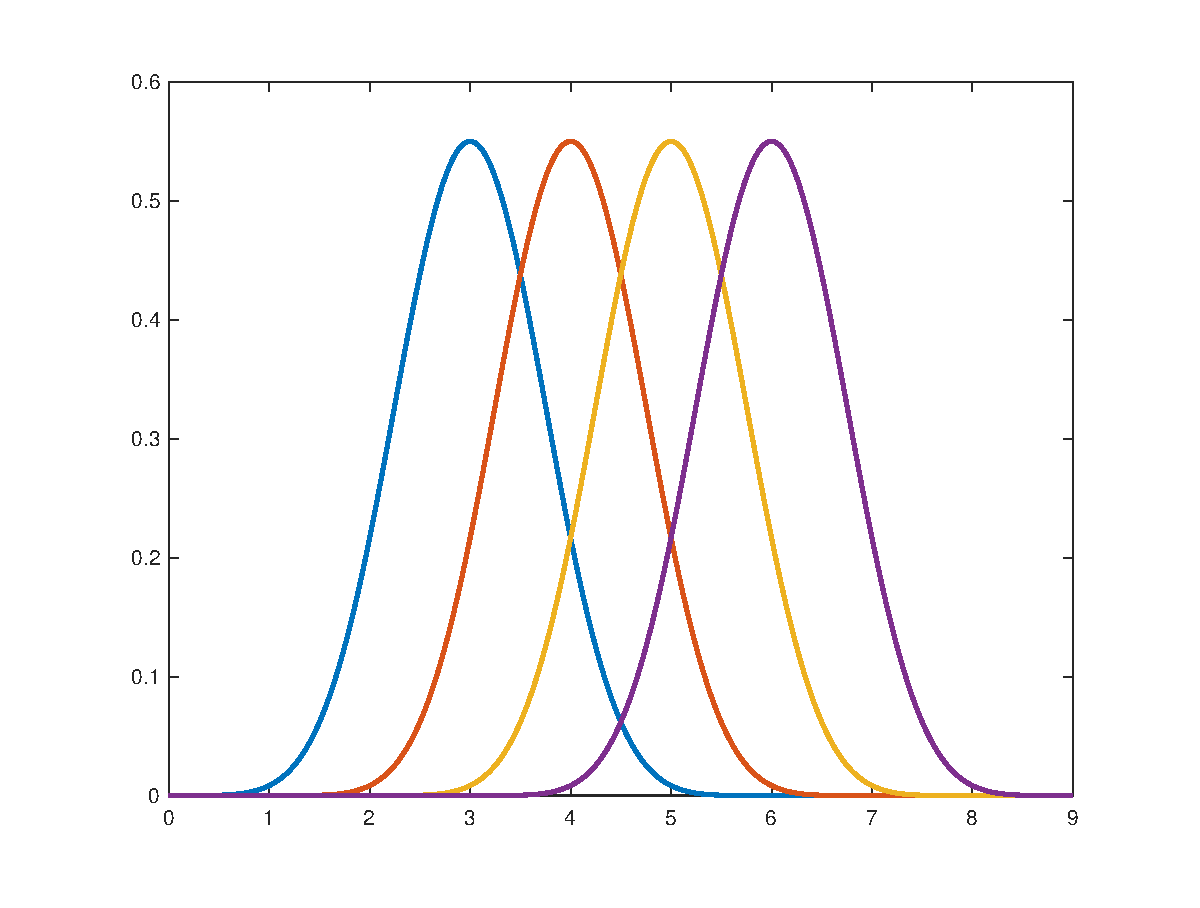
\includegraphics[width=\textwidth]{figure/6_41.eps}
    \caption{$\mathbf{t} = [0, 1, 2, 3, 4, 5, 6, 7, 8, 9]$}
    \label{fig:641}
  \end{subfigure}
  \begin{subfigure}[b]{0.3\textwidth}
      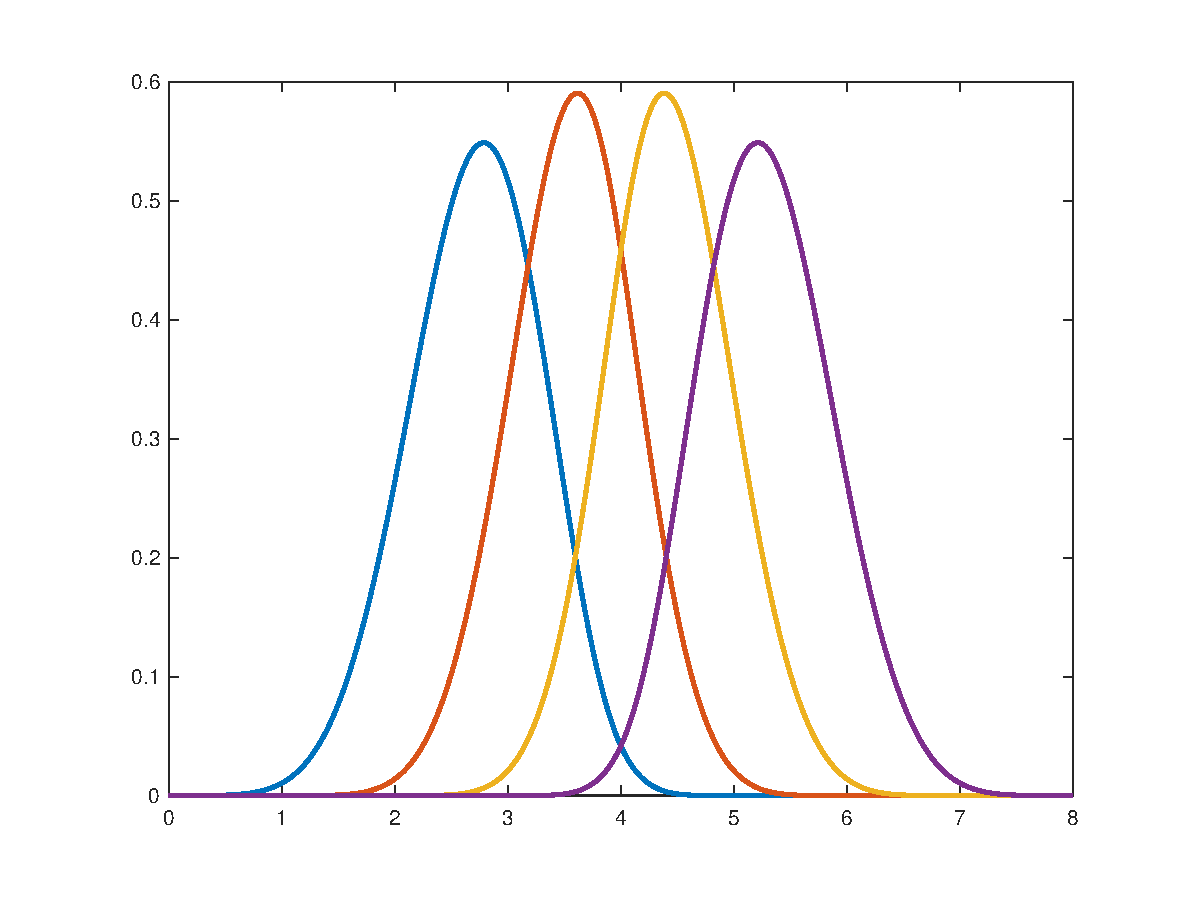
\includegraphics[width=\textwidth]{figure/6_42.eps}
      \caption{$\mathbf{t} = [0, 1, 2, 3, 4, 4, 5, 6, 7, 8]$}
      \label{fig:642}
  \end{subfigure}
  \begin{subfigure}[b]{0.3\textwidth}
      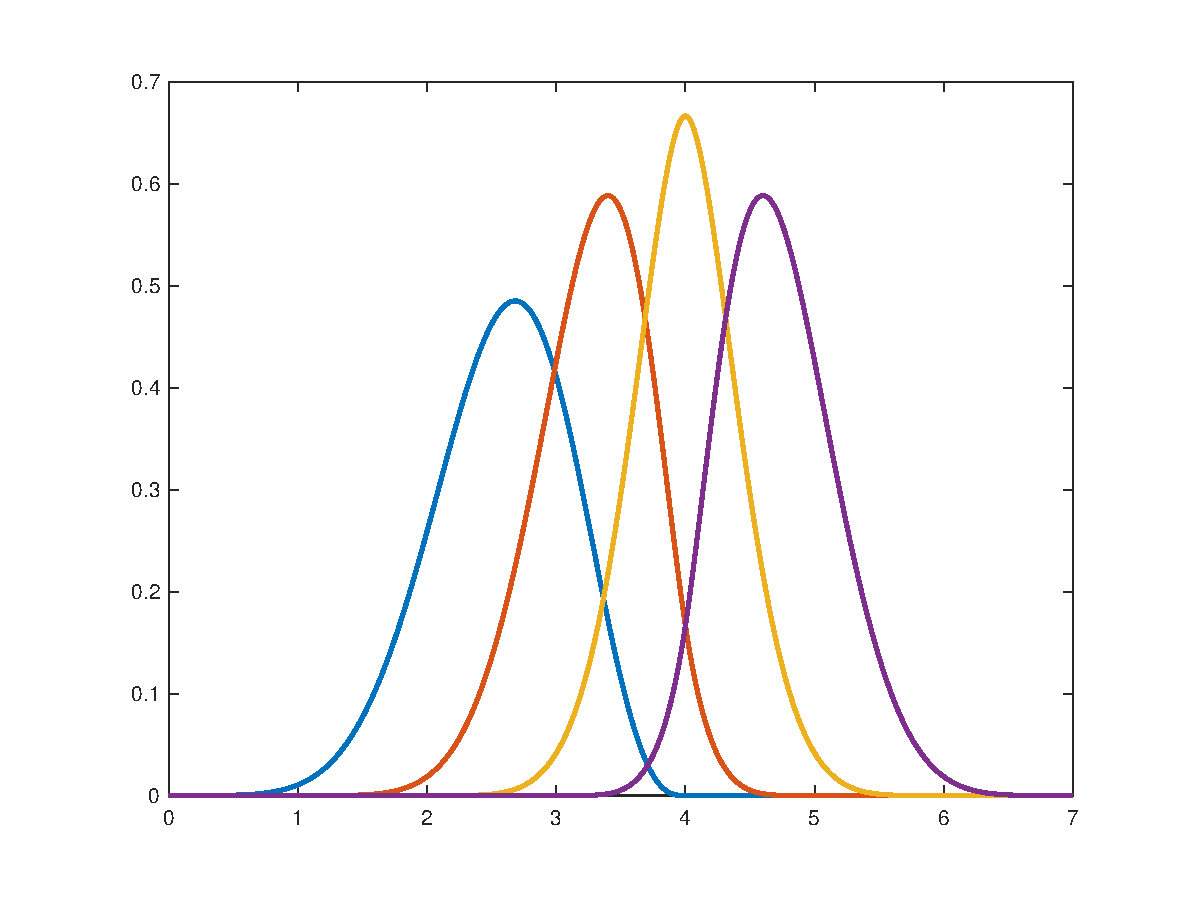
\includegraphics[width=\textwidth]{figure/6_43.eps}
      \caption{$\mathbf{t} = [0, 1, 2, 3, 4, 4, 4,5, 6, 7]$}
      \label{fig:643}
  \end{subfigure}
  \begin{subfigure}[b]{0.3\textwidth}
      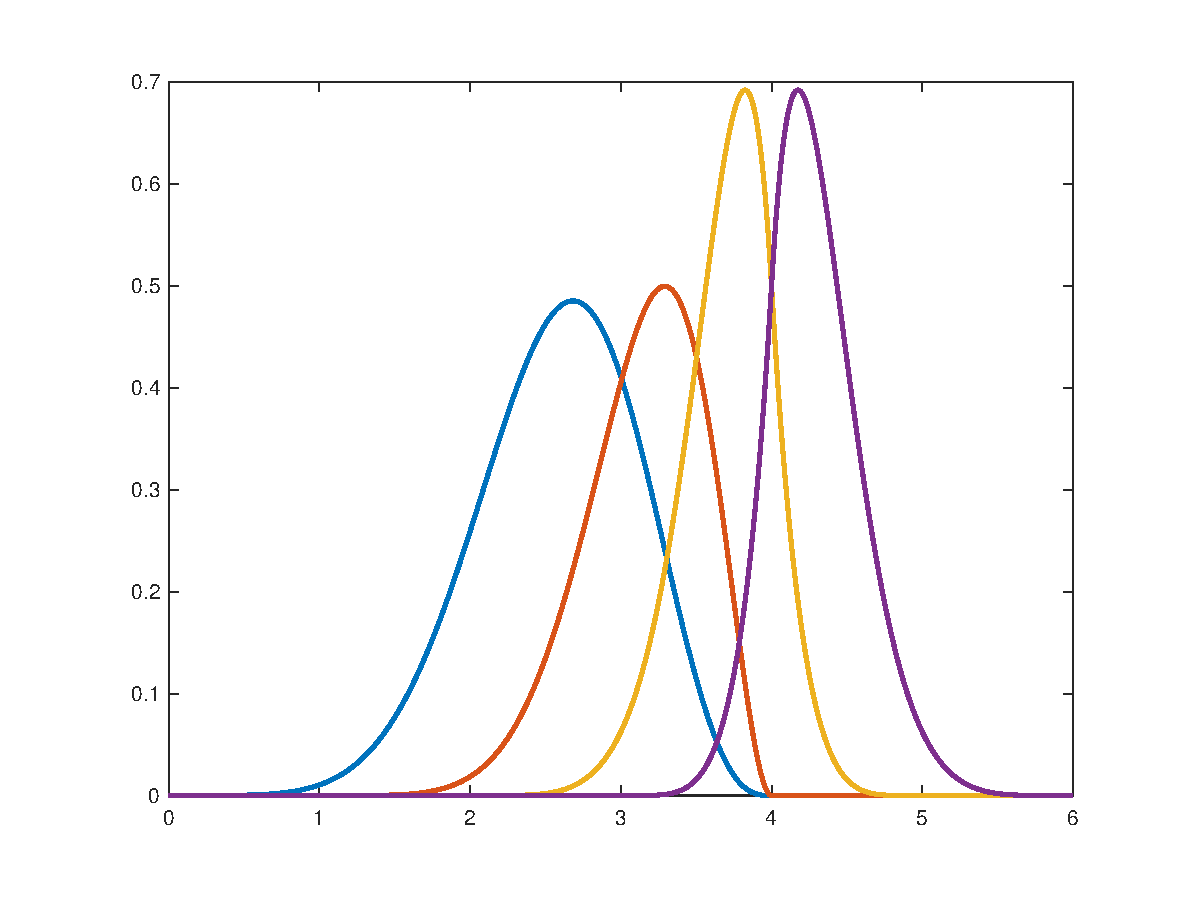
\includegraphics[width=\textwidth]{figure/6_44.eps}
      \caption{$\mathbf{t} = [0, 1, 2, 3, 4, 4, 4, 4, 5, 6]$}
      \label{fig:644}
  \end{subfigure}
  \begin{subfigure}[b]{0.3\textwidth}
    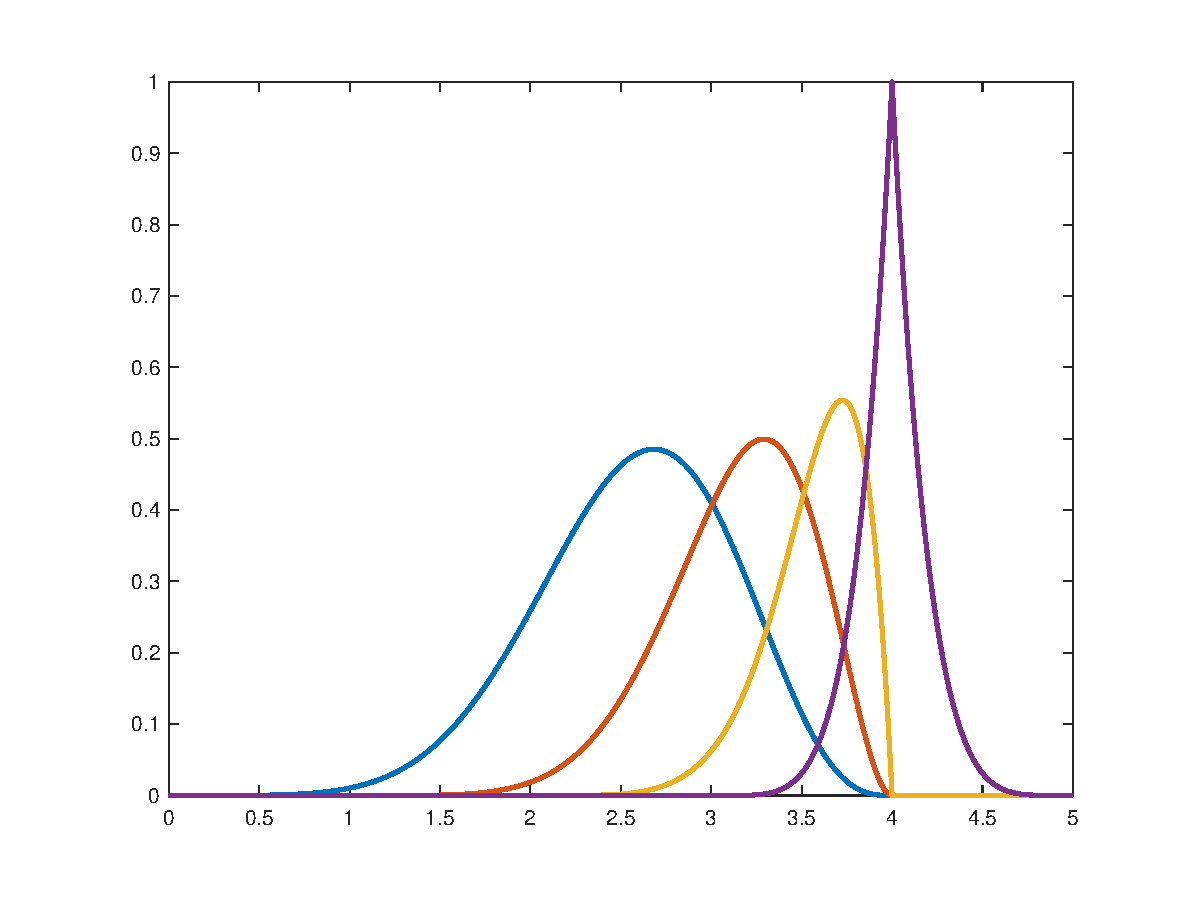
\includegraphics[width=\textwidth]{figure/6_45.eps}
    \caption{$\mathbf{t} = [0, 1, 2, 3, 4, 4, 4, 4, 5]$}
    \label{fig:645}
  \end{subfigure}
  \caption{Base con nodi multipli di ordine 6}\label{fig:animals}
\end{figure}

Un caso particolare della base delle B-Spline sono i polinomi di Bernstein. Questi ultimi si ottengono quando, 
dato $[a, b] = [\tau_0, \tau_L]$, la partizione nodale estesa è formata solamente da $a$ ripetuto $k$ volte
e $b$ ripetuto altrettante $k$ volte. In Figura~\ref{fig:bernstein} è mostrato un esempio di base ottenuta con 
i polinomi di Bernstein di grado $5$.

\begin{figure}[]
  \centering
  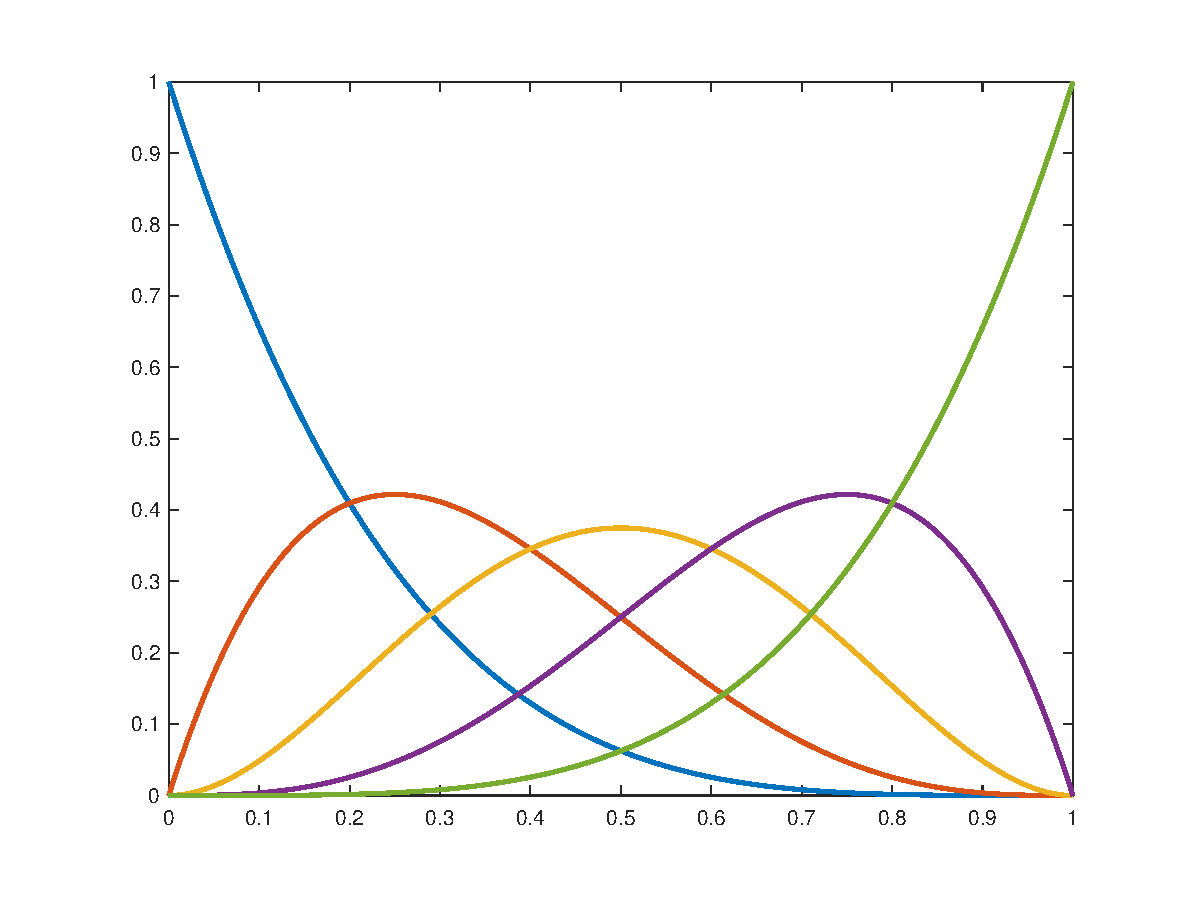
\includegraphics[width=0.75\textwidth]{figure/bernstein5_from_cox_de_boor.eps}
  \caption{Base di Bernstein di ordine $5$}
  \label{fig:bernstein}
\end{figure} 

\subsection{Proprietà della base delle B-Spline}
La base delle B-Spline gode di diverse proprietà:
\begin{enumerate}
  \item Supporto locale: $N_{i, r}(t) = 0 \text{ se } t \notin [t_i, t_{i+r}]$
  \item Non negatività: $N_{i, r}(t) \geq 0\ \forall \ t \ \in \mathbb{R}$
  \item Partizione dell'unità: $\sum_{i = 0}^{n+k-r} = 1 \ \forall \  t \ \in [t_{r-1}, t_{n+1+k-r}] \text{ con } r = 1 \dots k$
\end{enumerate}
\paragraph{Supporto locale}
Questa proprietà ci dice che la spline $N_{i, r}(t)$ è diversa da zero solamente nell'intervallo di nodi che va 
da $t_i$ a $t_{i+r}$. Prendiamo ad esempio le B-Spline di ordine $k = 4$ e 
con $\mathbf{t} = [0, 0, 0, 1, 1, 2, 3, 3, 3]$. Le splines saranno le seguenti:
\begin{itemize}
  \item $N_{1, 4}(t)\neq 0\ t \in [t_1 = 0, t_5 = 1]$
  \item $N_{2, 4}(t)\neq 0\ t \in [t_2 = 0, t_6 = 2]$
  \item $N_{3, 4}(t)\neq 0\ t \in [t_3 = 0, t_7 = 3]$
  \item $N_{4, 4}(t)\neq 0\ t \in [t_4 = 1, t_8 = 3]$
  \item $N_{5, 4}(t)\neq 0\ t \in [t_5 = 1, t_9 = 3]$
\end{itemize}
Facendo un plot di questa base possiamo vedere come la proprietà di supporto locale sia verificata, in particolare in Figura~\ref{fig:local_support} sono mostrate
tutte le splines della base, mentre in Figura~\ref{fig:first_property} è mostrato un dettaglio della $N_{1, 4}(t)$ per $t = [0.85, 1.15]$.
\begin{figure}[]
  \centering
  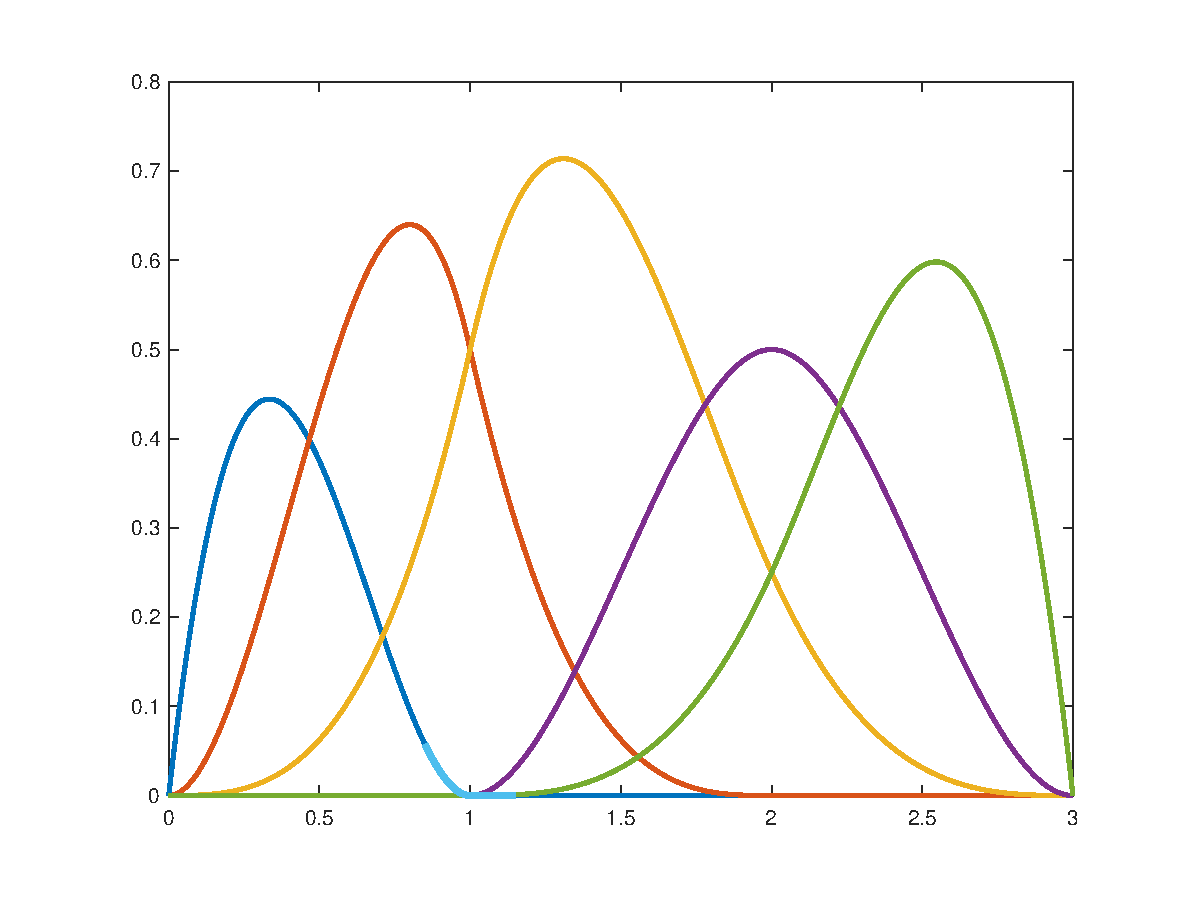
\includegraphics[width=0.75\textwidth]{figure/local_support.eps}
  \caption{Supporto locale}
  \label{fig:local_support}
\end{figure} 
\begin{figure}[]
  \centering
  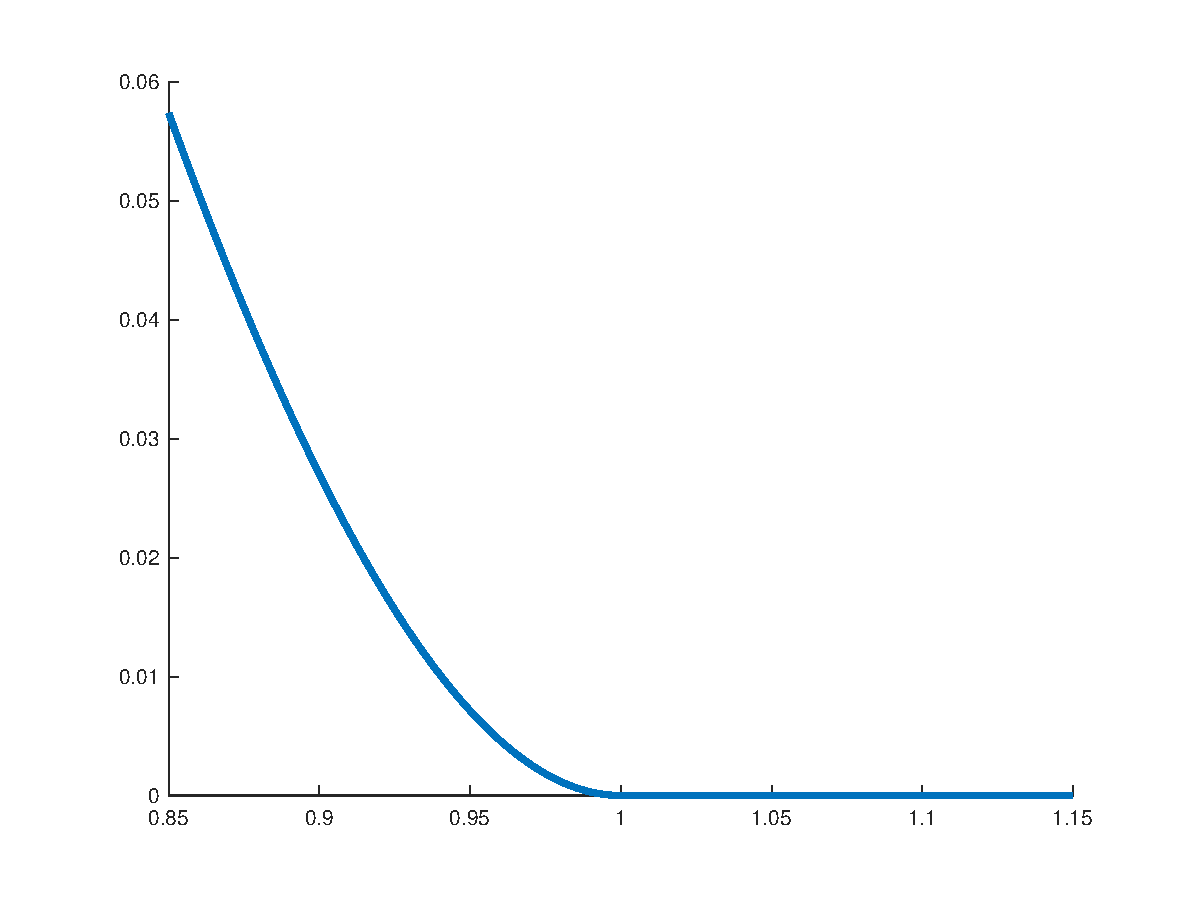
\includegraphics[width=0.75\textwidth]{figure/first_property.eps}
  \caption{Dettaglio della prima splines $N_{1, 4}(t)$ per $t = [0.85, 1.15]$}
  \label{fig:first_property}
\end{figure} 
\paragraph{Non negatività} In questo caso la proprietà è facilmente verificabile sfruttando uno qualunque dei plot mostrati in precedenza,
 ad esempio possiamo vedere che in Figura \ref{fig:local_support} nessuna delle $N_{i, r}(t)$ è negativa.
\paragraph{Partizione dell'unità} BONA
\begin{figure}[]
  \centering
  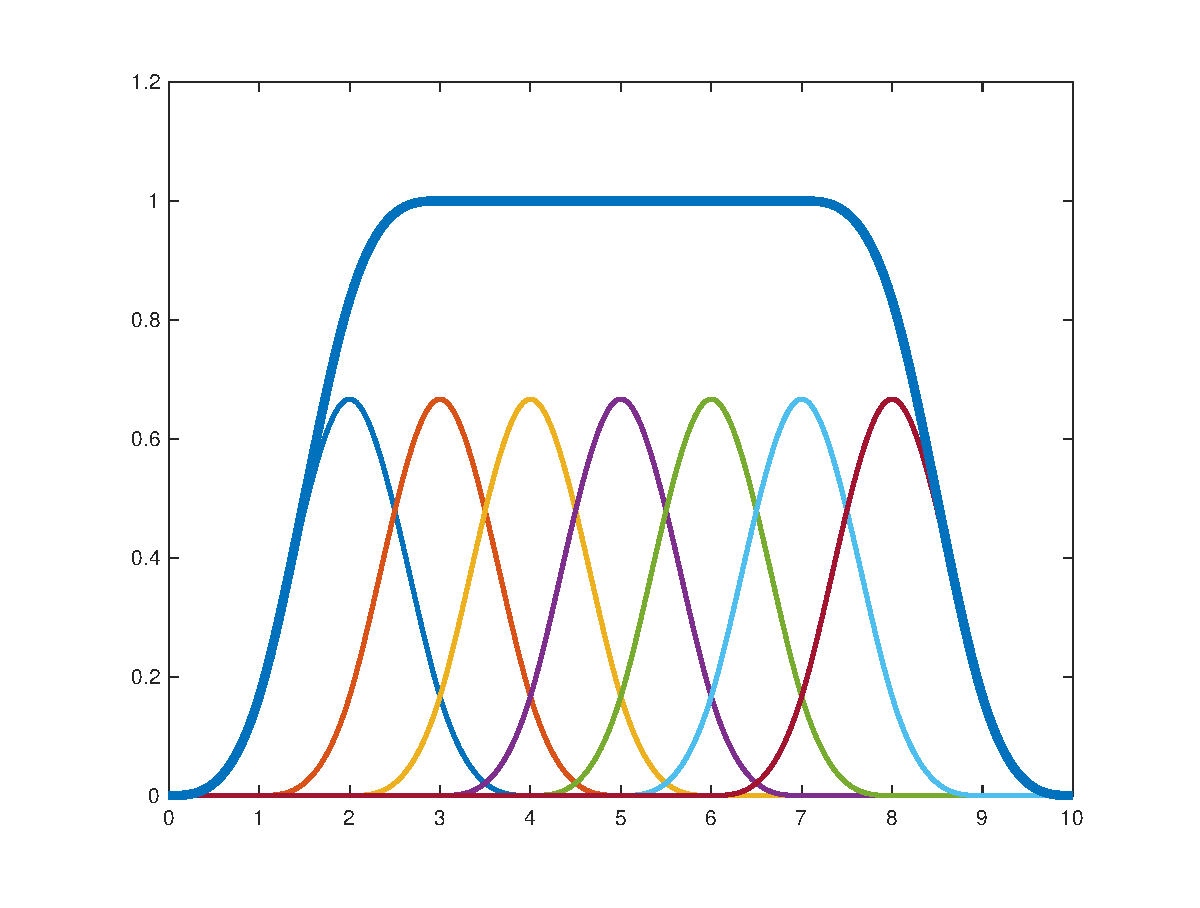
\includegraphics[width=0.75\textwidth]{figure/unity_std.eps}
  \caption{Partizione dell'unità con nodi uniformi}
  \label{fig:unity_std}
\end{figure} 
\begin{figure}[]
  \centering
  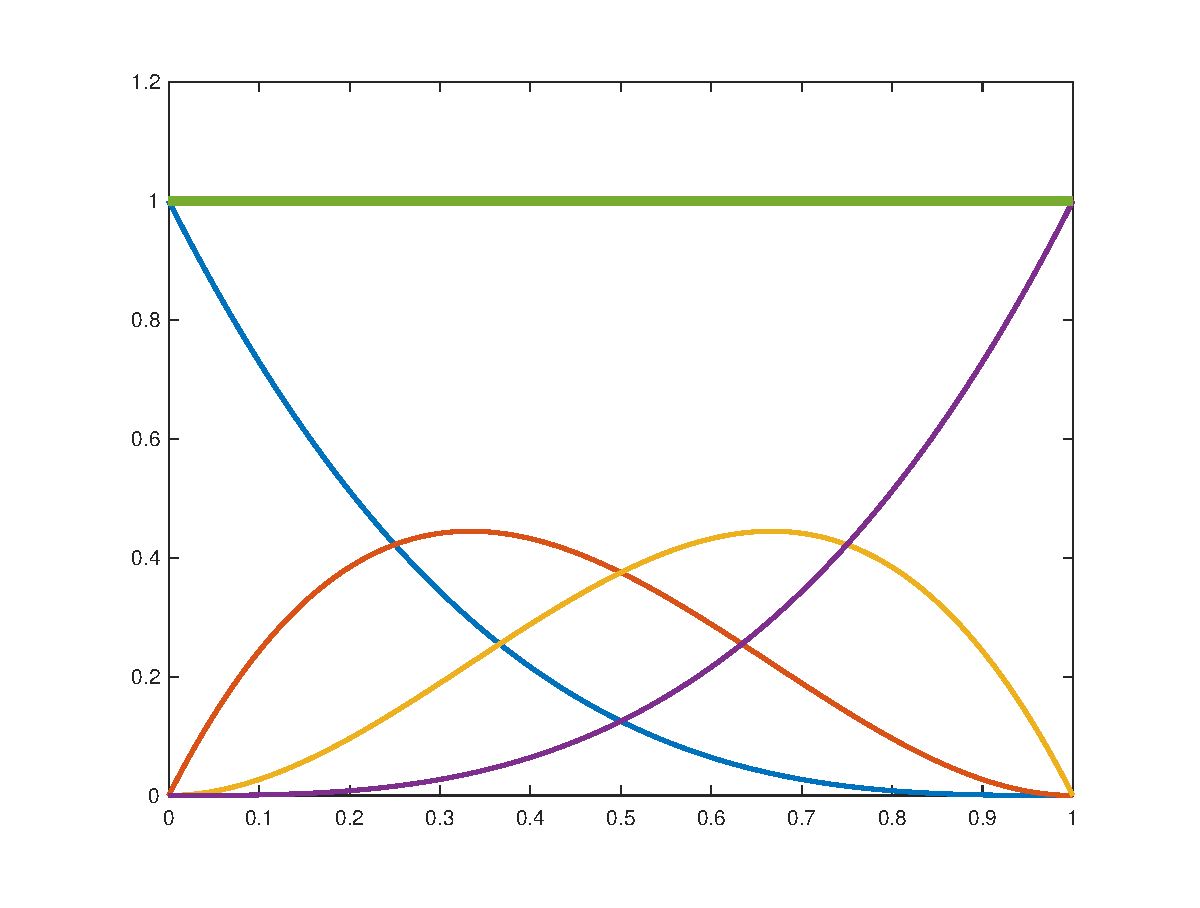
\includegraphics[width=0.75\textwidth]{figure/unity_bernstein.eps}
  \caption{Partizione dell'unità nella base di Bernstein}
  \label{fig:unity_bernstein}
\end{figure} 
\begin{figure}[]
  \centering
  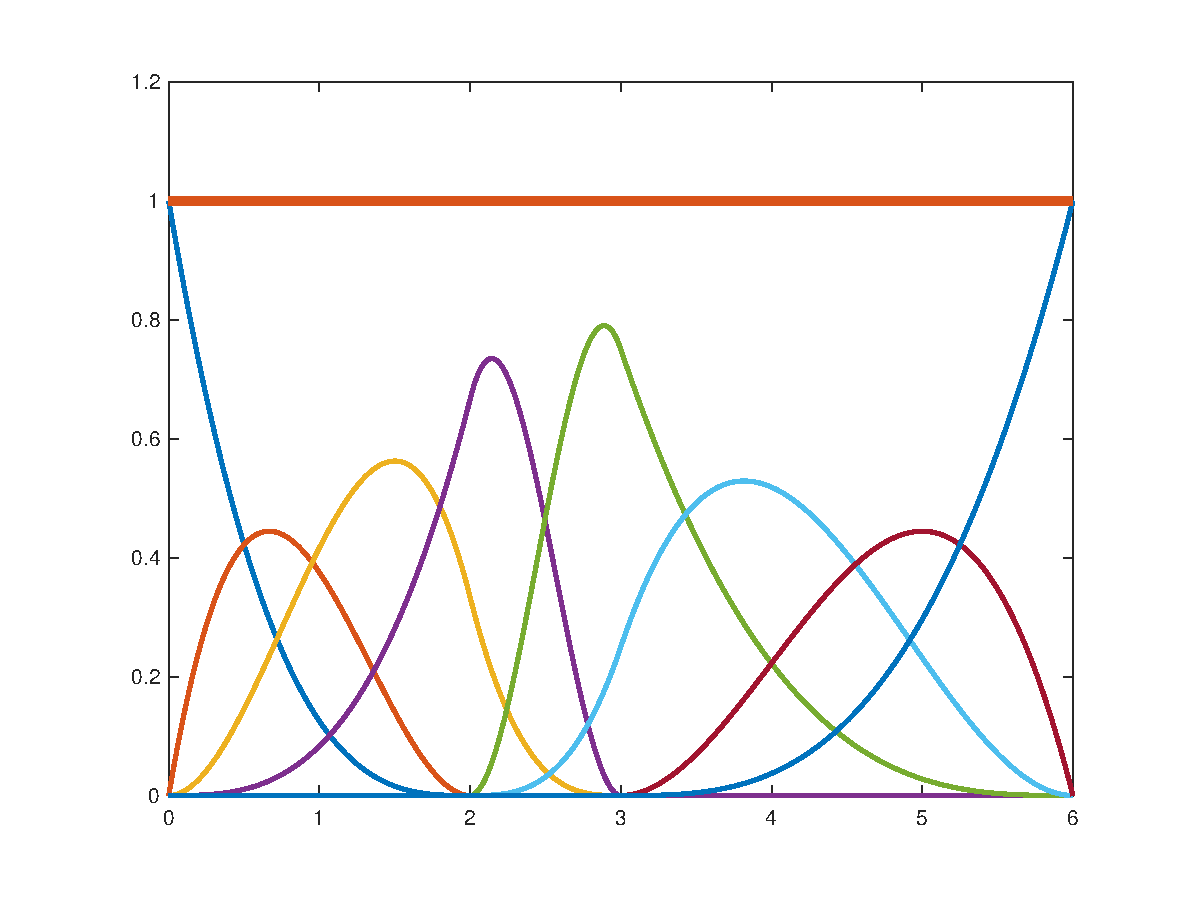
\includegraphics[width=0.75\textwidth]{figure/unity_3.eps}
  \caption{Partizione dell'unità con partizione nodale \textit{clamped}}
  \label{fig:unity_clamped}
\end{figure} 


\section{Curve B-Spline}
A partire dalla base delle B-Spline è possibile realizzare delle curve. Dati $n+1$ punti 
di controllo la curva è definita come 
$$\mathbf{X}(t) := \sum_{i=0}^{n} \mathbf{d_i} N_{i, k}(t)$$

\subsection{Proprietà delle curve B-Spline}
Le curve B-Spline godono di diverse proprietà:
\begin{enumerate}
  \item Invarianza per trasformazioni affini: la proprietà della base delle B-Spline di essere 
  una partizione dell'unità garantisce che le curve B-Spline siano invarianti per trasformazioni affini, questo 
  vuol dire che applicare la trasformazione affine sulla curva, o sui punti di controllo è indifferente in quanto il risultato non cambia.
  \item Località: un segmento di curva è influenzato solamente da $k$ punti di controllo.
  \item Strong Convex Hull: ogni punto sulla curva appartiene all'inviluppo convesso di $k$ punti di controllo consecutivi, con $k$ ordine 
  delle funzioni spline.
  \item Variation Diminishing: il numero di intersezioni tra una retta e la curva è minore o uguale al numero di intersezioni
  tra la stessa retta ed il poligono di controllo.
\end{enumerate}



\paragraph{Invarianza per trasformazioni affini} In Codice~\ref{code:trasnformationspline} è 
presente il codice con cui è stata applicata una trasformazione
prima ai punti di controllo e poi alla curva. Come si può vedere dal 
Codice~\ref{code:trasnformationspline} la 
trasformazione applicata è stata una rotazione di $180$ gradi
ed uno spostamento di $1$ su entrambi gli assi. Per generare la base con cui poi è 
stata disegnata la curva è stata usata la funzione \texttt{spcol} del \textit{Curve Fitting Toolbox}.
Un modo \textit{Naïve} con cui ci si può accertare della veridicità di questa proprietà è 
guardando il Codice~\ref{code:trasnformationspline} e la Figura~\ref{fig:trasformationspline}; nel codice sono presenti 
tre chiamate a funzione \texttt{plot}: la prima per la curva originale, la seconda per la curva sulla quale è
stata applicata la trasformazione e la terza per la curva disegnata a partire dai punti di controllo
sui quali è stata applicata la trasformazione. Si può però osservare che nella Figura~\ref{fig:trasformationspline} sono presenti due curve, 
ciò vuol dire che
due curve si sono sovrapposte.
\begin{figure}[]
  \centering
  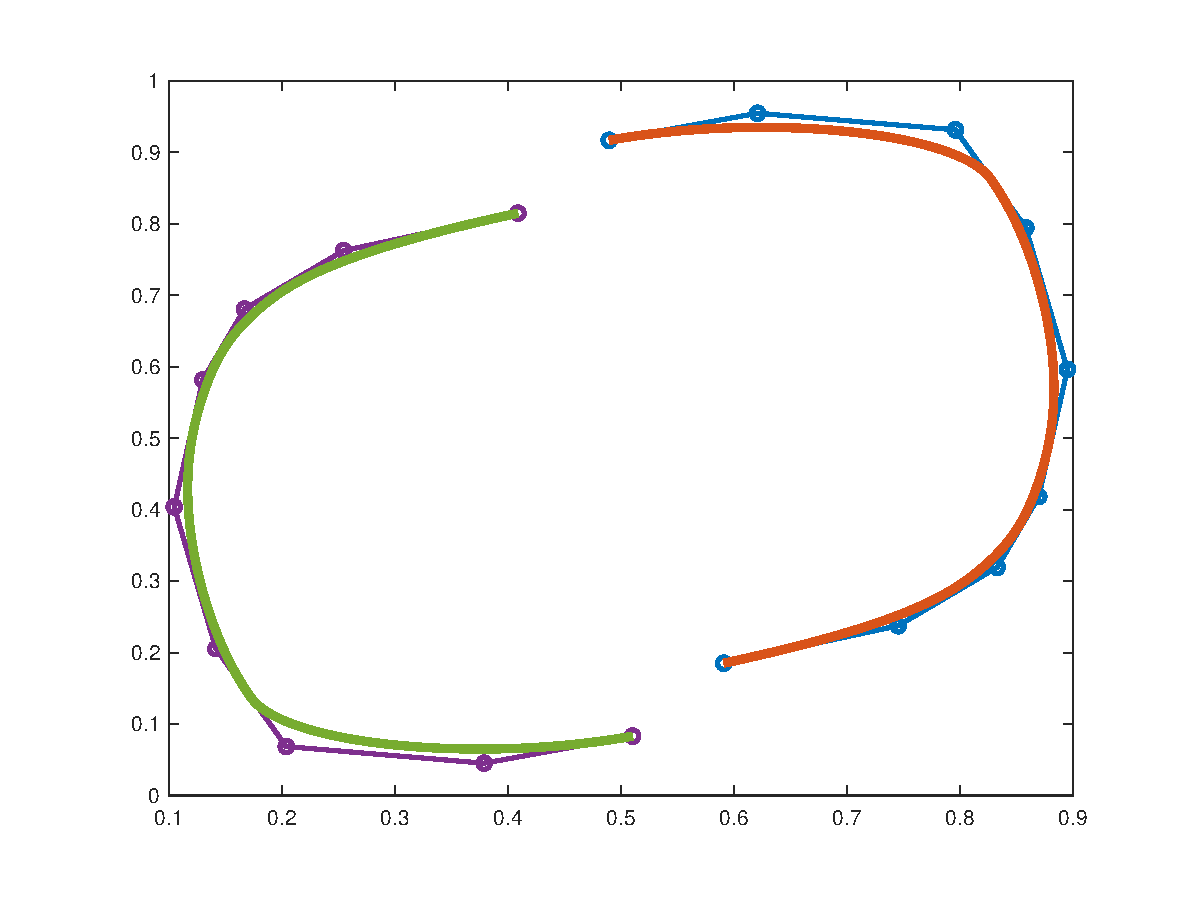
\includegraphics[width=0.75\textwidth]{figure/transformation_spline.eps}
  \caption{Trasformazione affine su spline}
  \label{fig:trasformationspline}
\end{figure} 
\lstinputlisting[label=code:trasnformationspline, firstline=2, language=Matlab, caption = Applicazone trasformazione affine]{code/b_spline_curve_prop_trans.m}



\paragraph{Località} La proprietà di località ci dice  che il punto di controllo $\mathbf{d_j}$ influenza la curva solamente per $t \in [t_j, t_{j+k}]$. 
Ad esempio, come mostrato in Figura~\ref{fig:loc_spline1} ed in Codice~\ref{code:locspline}, spostando $\mathbf{d}_7$ la curva varia da $t \in [t_7, t_{11}]$. 


\begin{figure}[]
  \centering
  \begin{subfigure}[b]{0.3\textwidth}
    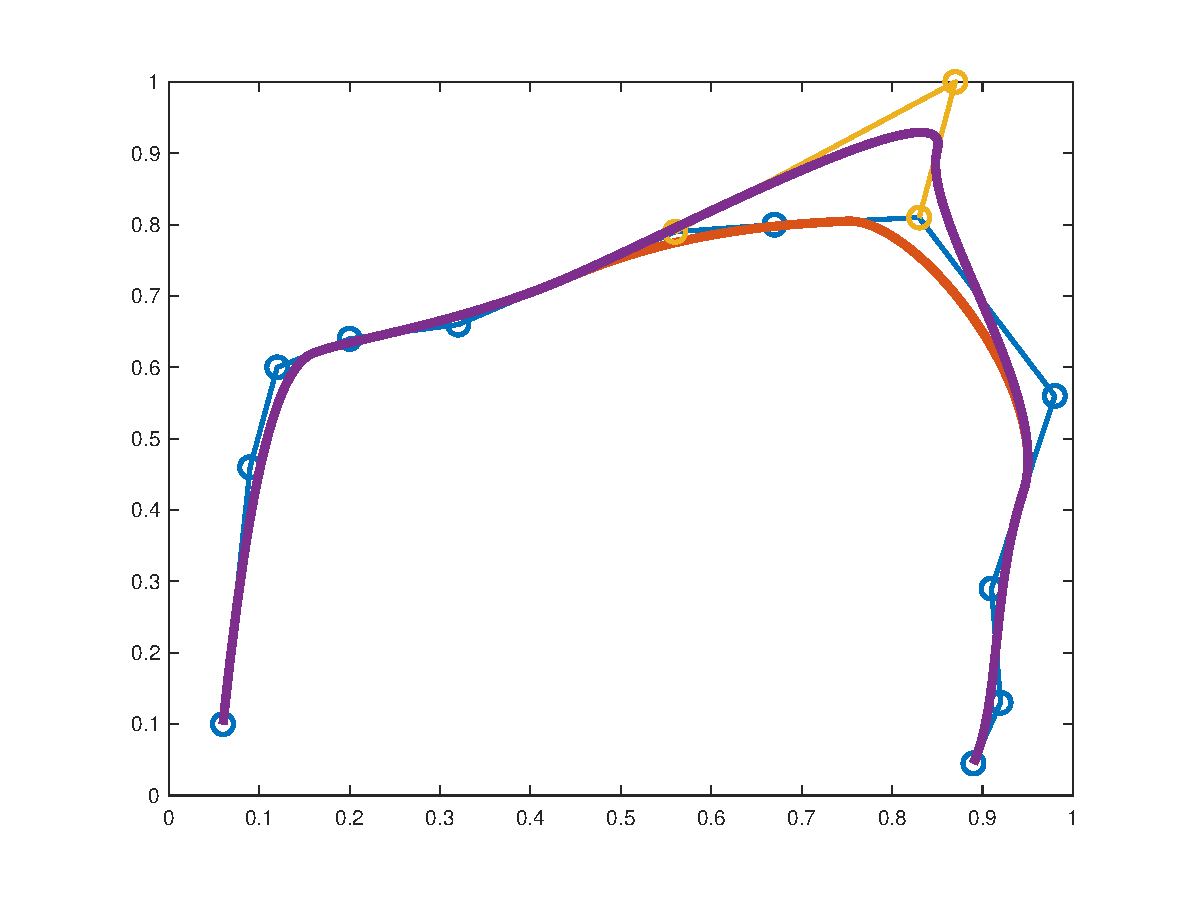
\includegraphics[width=\textwidth]{figure/loc3.eps}
    \caption{Spostamento di $\mathbf{d_7}$ }
    \label{fig:loc3}
  \end{subfigure}
  \begin{subfigure}[b]{0.3\textwidth}
      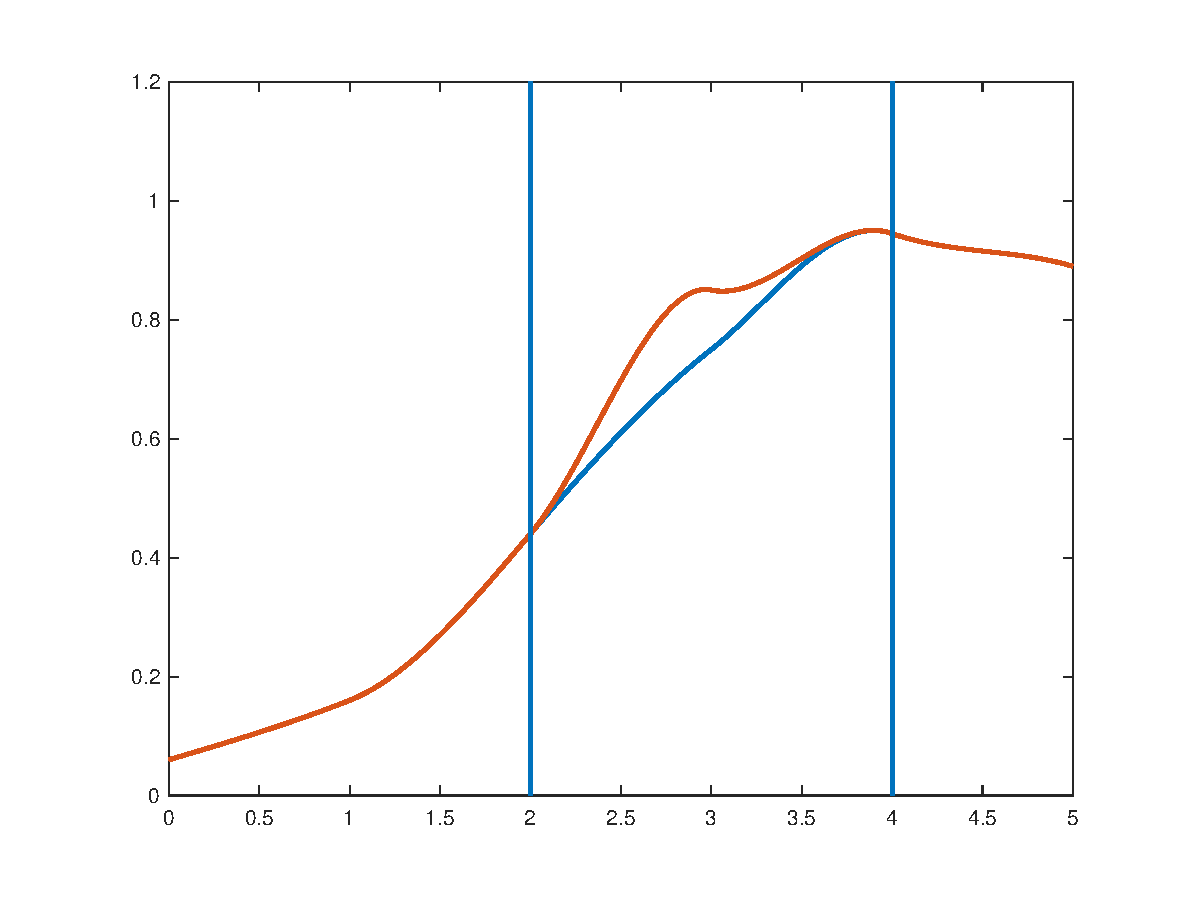
\includegraphics[width=\textwidth]{figure/loc2.eps}
      \caption{Variazione sulla $x$}
      \label{fig:loc2}
  \end{subfigure}
  \begin{subfigure}[b]{0.3\textwidth}
      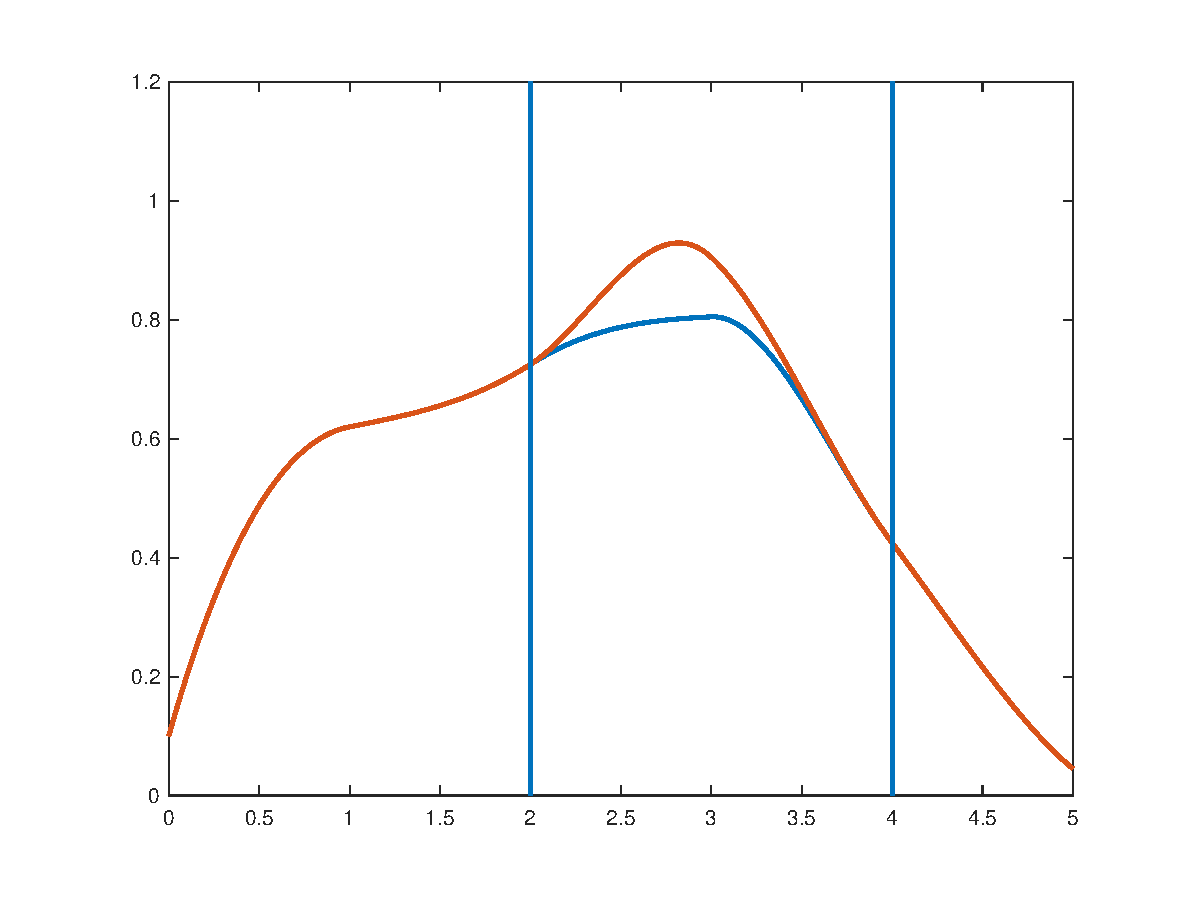
\includegraphics[width=\textwidth]{figure/loc1.eps}
      \caption{Variazione sulla $y$}
      \label{fig:loc1}
  \end{subfigure}
  \caption{Proprietà di località}\label{fig:loc_spline1}
\end{figure}
\lstinputlisting[label=code:locspline, firstline=2, lastline = 33, language=Matlab, caption = Proprietà di località]{code/b_spline_curve_prop_loc.m}
La proprietà di località ci dice anche che una curva B-Spline $\mathbf{X}(t^*)$ con $t^* \in [t_r, t_{r+1})$ è determinata da 
$k$ punti di controllo $d_{r-k+1}, \dots, d_{r}$. 
Utilizzando Codice~\ref{code:locspline1} viene mostrata questa proprietà. Per questo esempio è stato scelto
$r = 8$, ed una partizione nodale mostrata a Riga 2 del Codice~\ref{code:locspline}.
I  punti di controllo spostati sono $8$, ovvero i $\mathbf{d}_j \notin [\mathbf{d}_{5}, \mathbf{d}_{8}]$.
Come mostrato in Figura~\ref{fig:loc_spline1} la curva  $\mathbf{X}(t^*)$  rimane quindi invariata per $t^* \in [t_{8}, t_{9})$. 

\lstinputlisting[label=code:locspline1, firstline=36, language=Matlab, caption = Proprietà di località]{code/b_spline_curve_prop_loc.m}



\begin{figure}[]
  \centering
  \begin{subfigure}[b]{0.3\textwidth}
    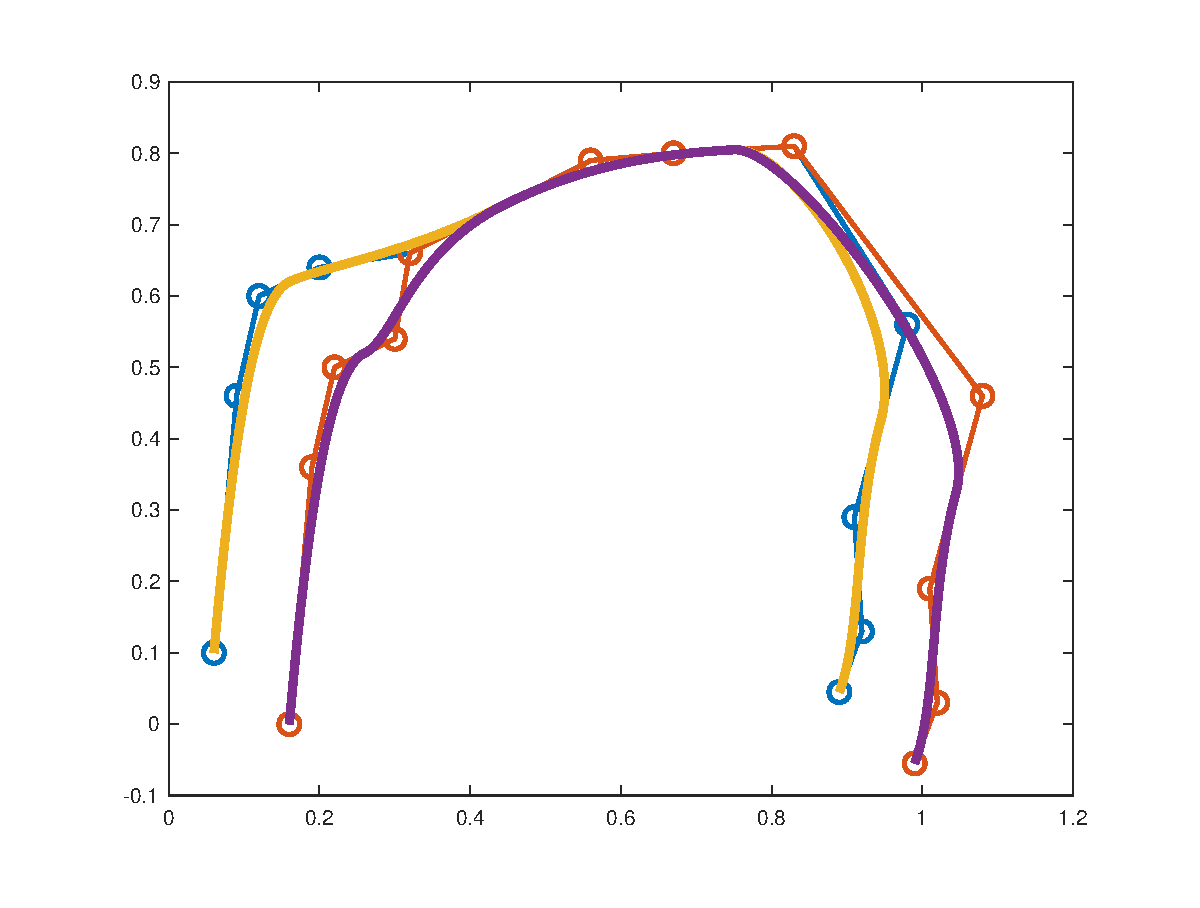
\includegraphics[width=\textwidth]{figure/loc6.eps}
    \caption{Spostamento di $\mathbf{d}_j \notin [\mathbf{d}_{5}, \mathbf{d}_{8}]$ }
    \label{fig:loc6}
  \end{subfigure}
  \begin{subfigure}[b]{0.3\textwidth}
      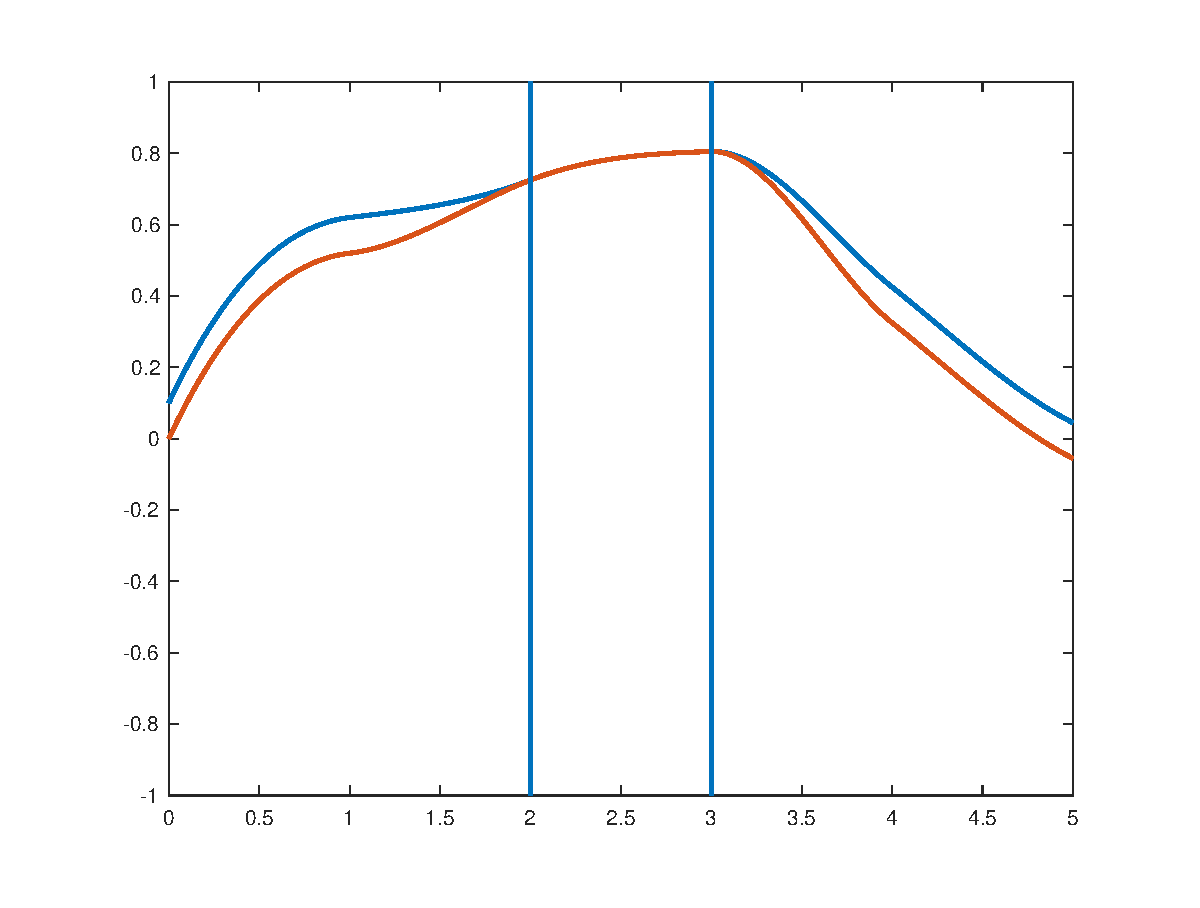
\includegraphics[width=\textwidth]{figure/loc5.eps}
      \caption{Variazione sulla $x$}
      \label{fig:loc5}
  \end{subfigure}
  \begin{subfigure}[b]{0.3\textwidth}
      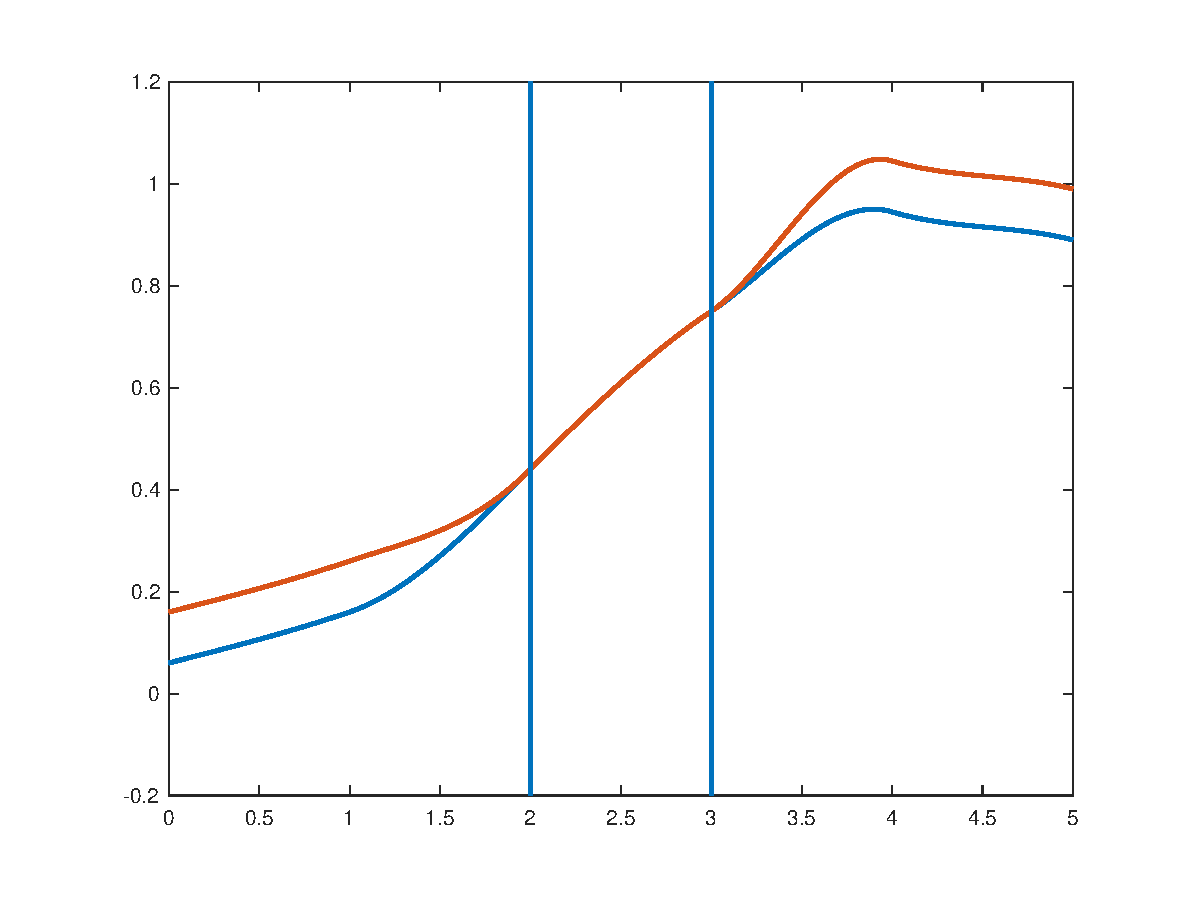
\includegraphics[width=\textwidth]{figure/loc4.eps}
      \caption{Variazione sulla $y$}
      \label{fig:loc4}
  \end{subfigure}
  \label{fig:loc_spline}
\end{figure} 

\paragraph{Strong Convex Hull}

TODO: CODICE, FIGURE, SCRIVERE

\paragraph{Variation Diminishing}
La proprietà di Variation Diminishing dice semplicemente che presa una qualunque retta che interseca
un numero $b$ di volte il poligono di controllo, questa intersecherà un numero di volte $a \leq b$ la curva \textit{B-Spline} 
disegnata a partire dal poligono di controllo. 
Un esempio realizzato con il Codice~\ref{code:vardim} è mostrato in Figura~\ref{fig:intersection}.
\lstinputlisting[label=code:vardim, firstline=2, language=Matlab, caption = Proprietà di Variation Diminishing]{code/b_spline_curve_prop_var_dim.m}
\begin{figure}[]
  \centering
  \begin{subfigure}[b]{0.3\textwidth}
    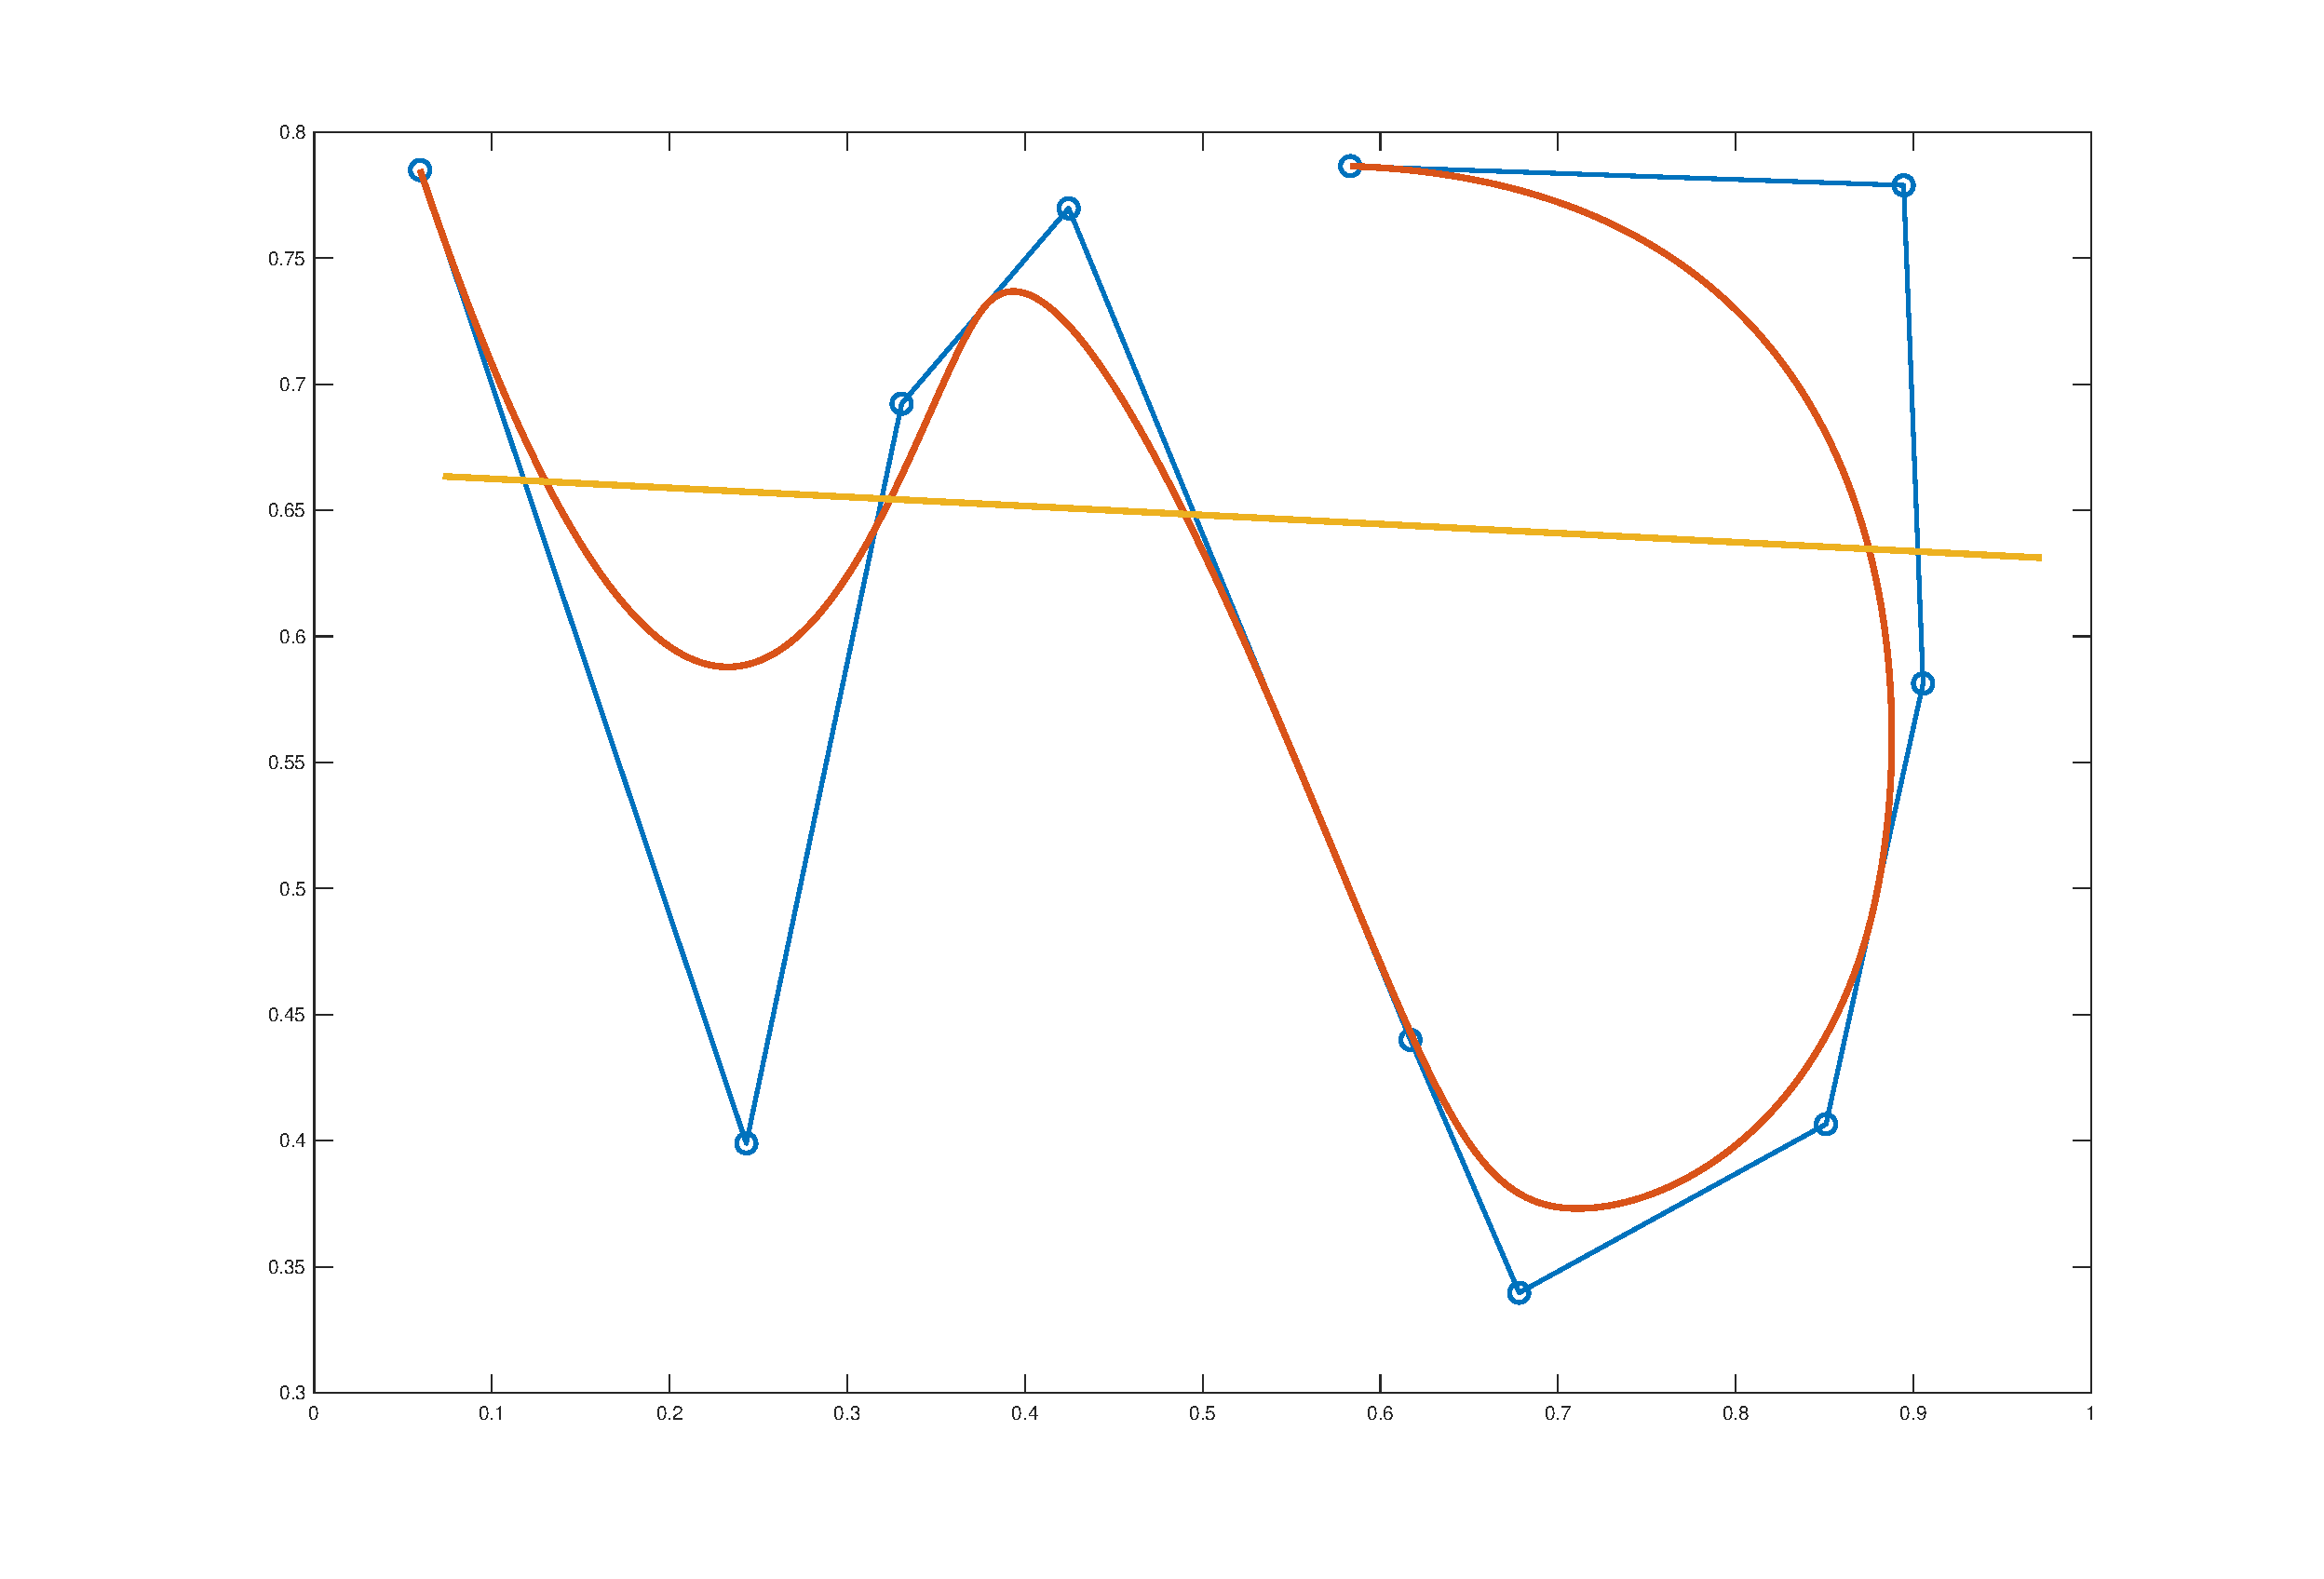
\includegraphics[width=\textwidth]{figure/intersection1.eps}
    \caption{Poligono: $4$, Curva: $4$}
    \label{fig:intersection1}
  \end{subfigure}
  \begin{subfigure}[b]{0.3\textwidth}
      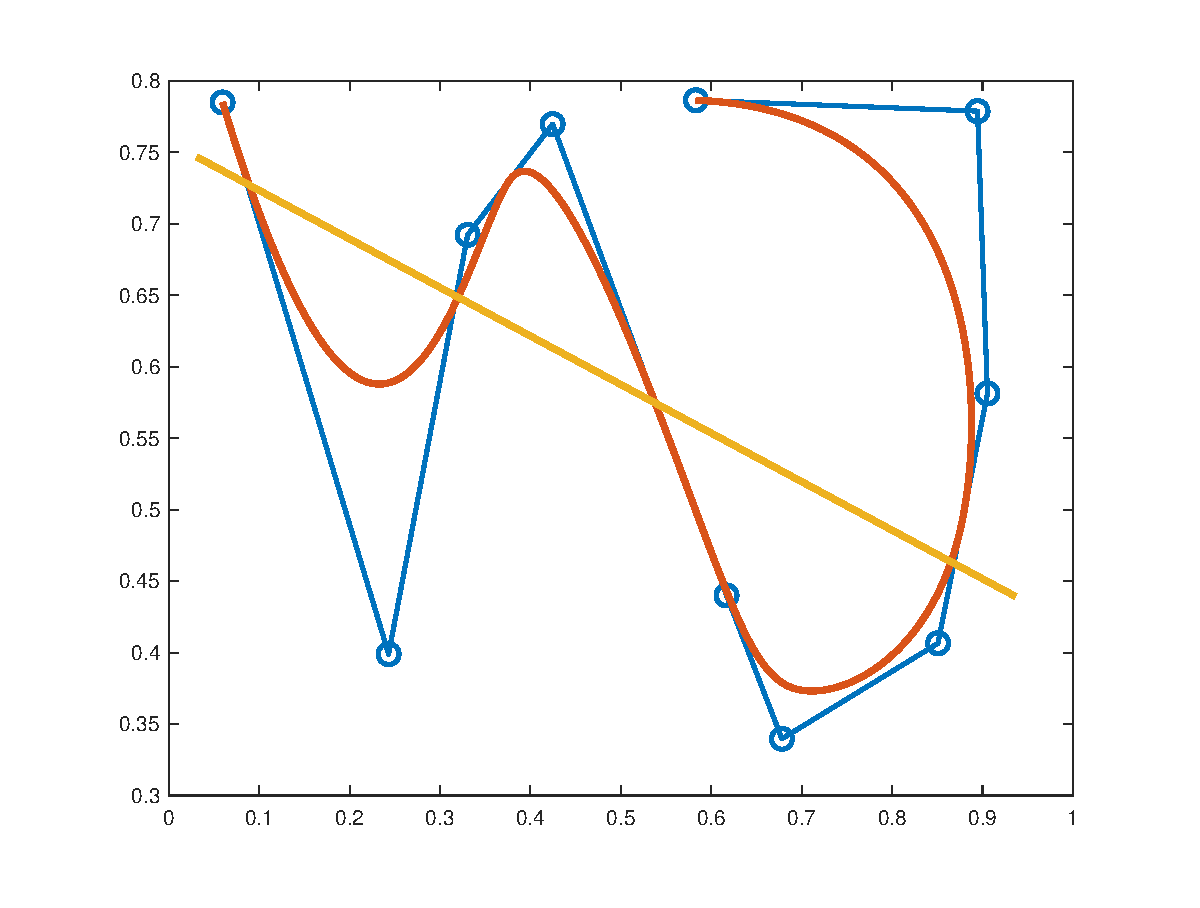
\includegraphics[width=\textwidth]{figure/intersection3.eps}
      \caption{Poligono: $4$, Curva: $4$}
      \label{fig:intersection3}
  \end{subfigure}
  \begin{subfigure}[b]{0.3\textwidth}
      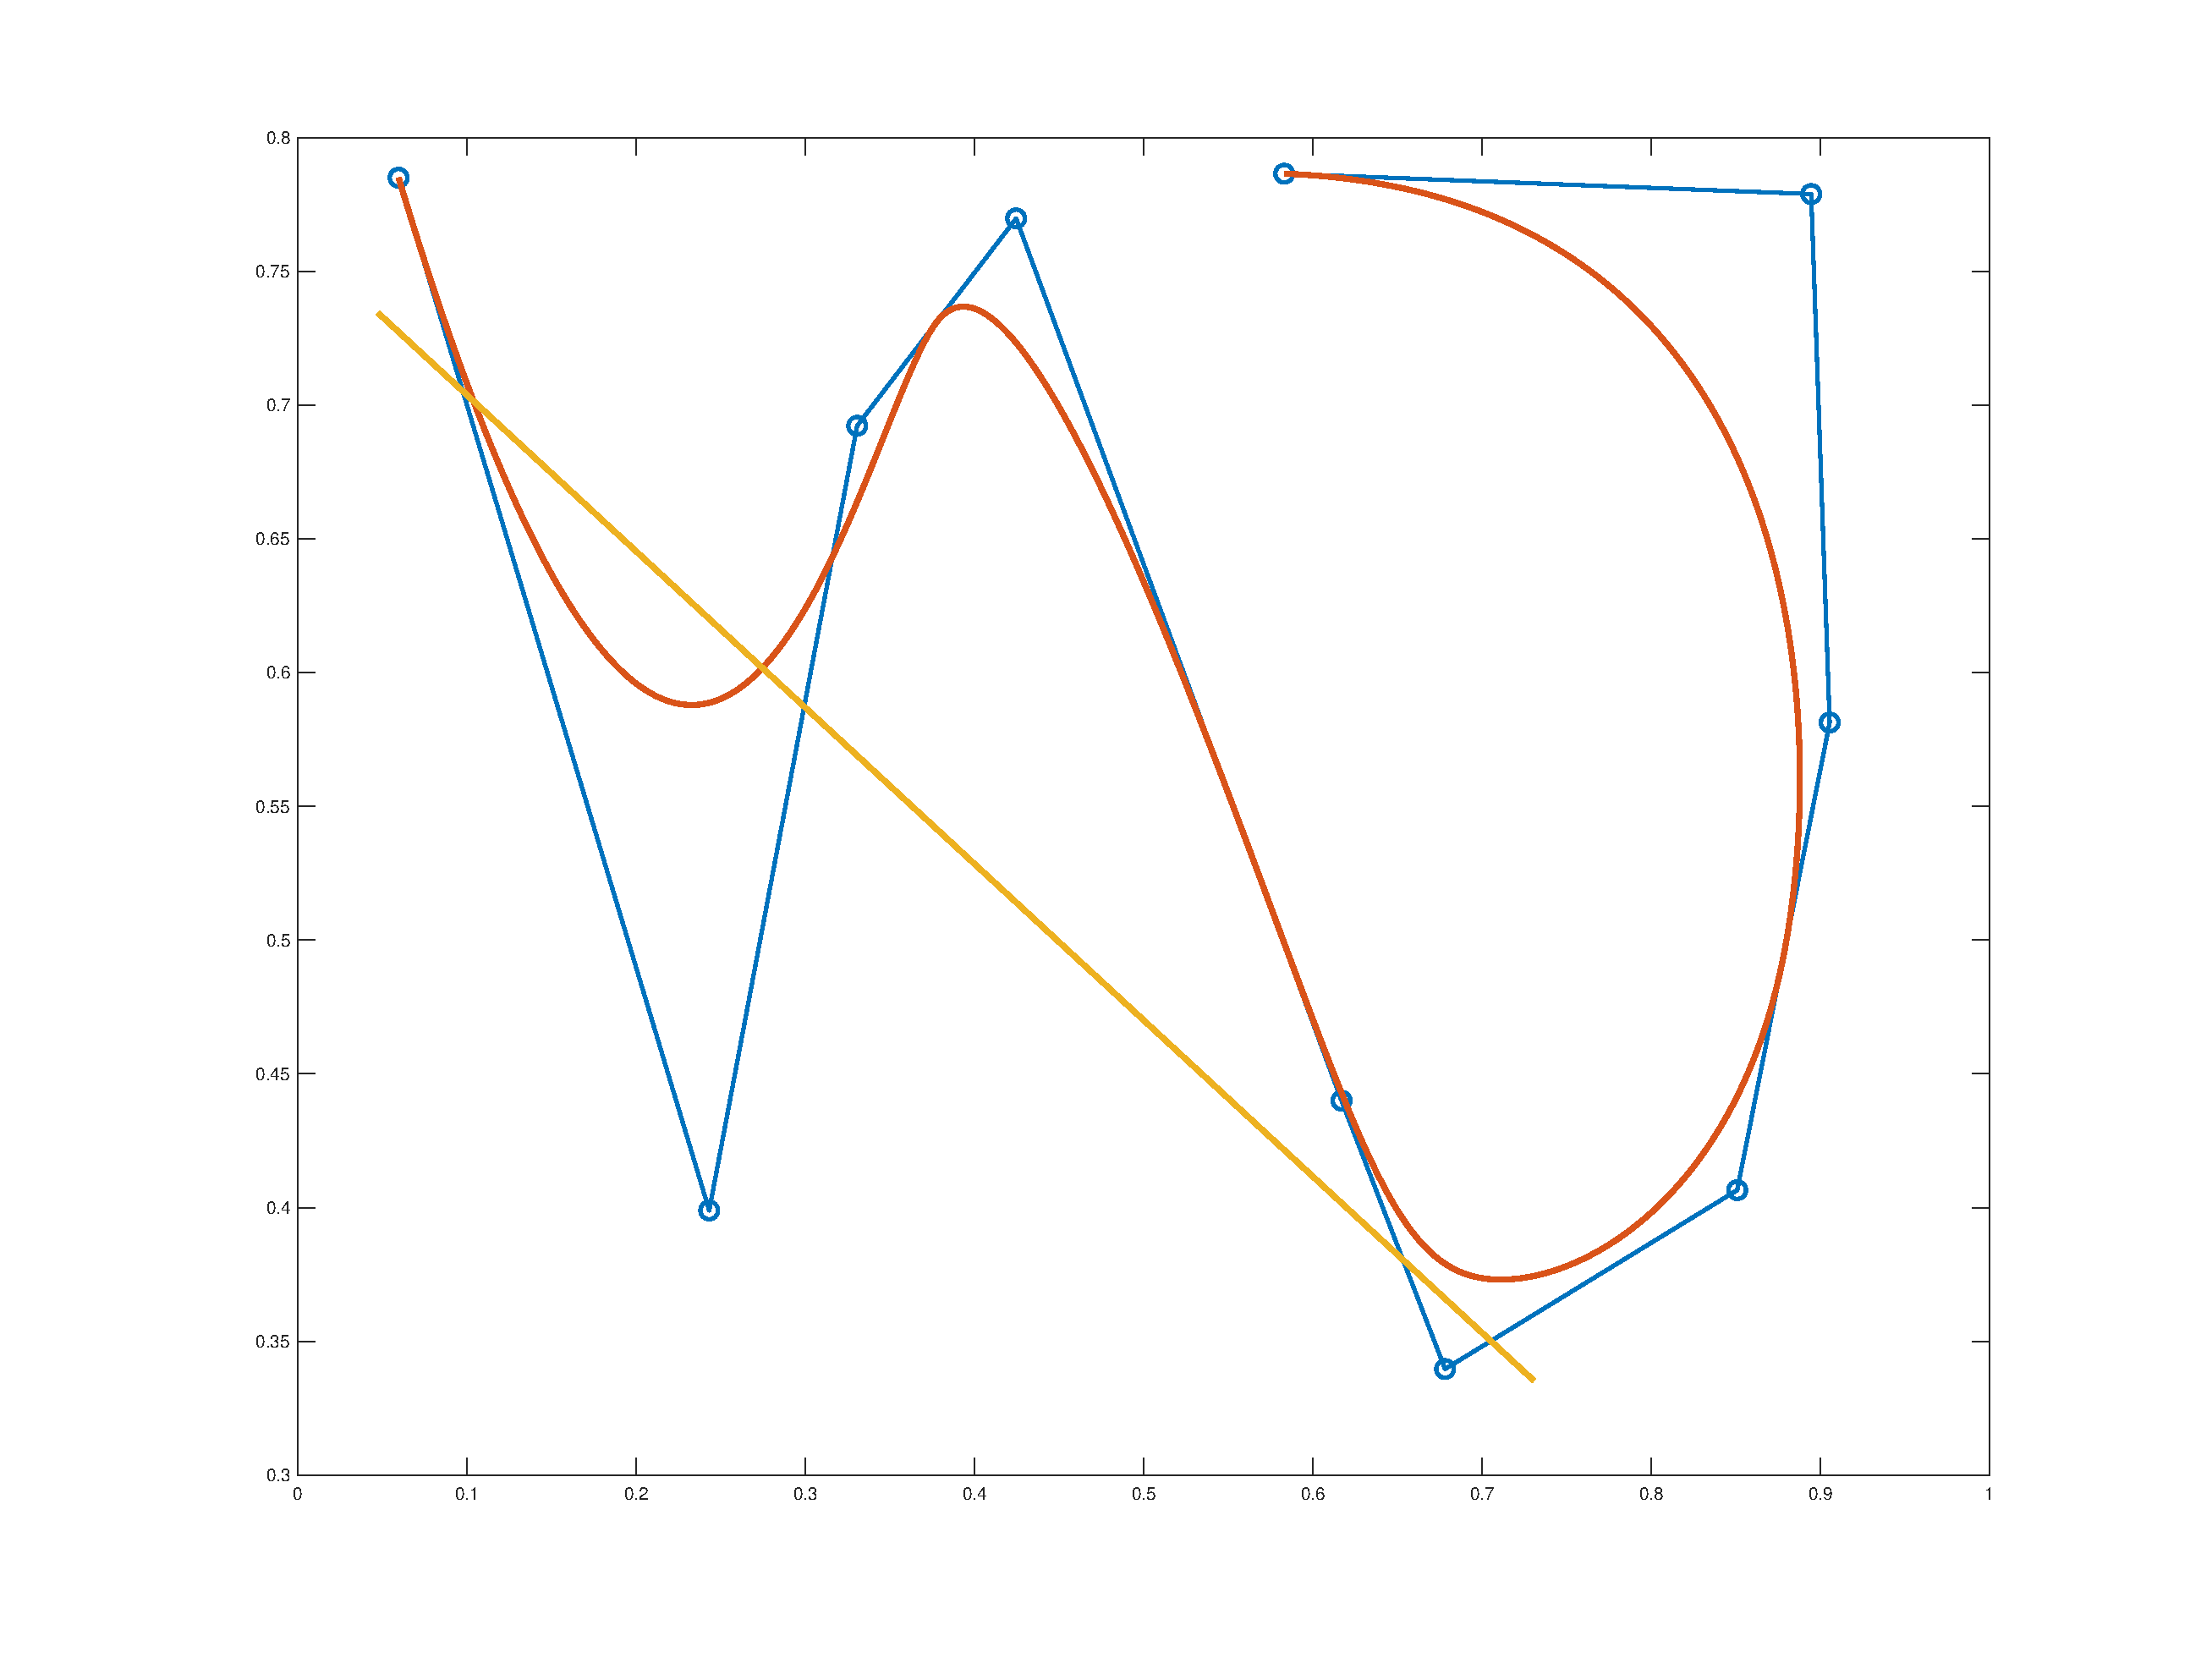
\includegraphics[width=\textwidth]{figure/intersection4.eps}
      \caption{Poligono: $4$, Curva: $2$}
      \label{fig:intersection4}
  \end{subfigure}
  \begin{subfigure}[b]{0.3\textwidth}
    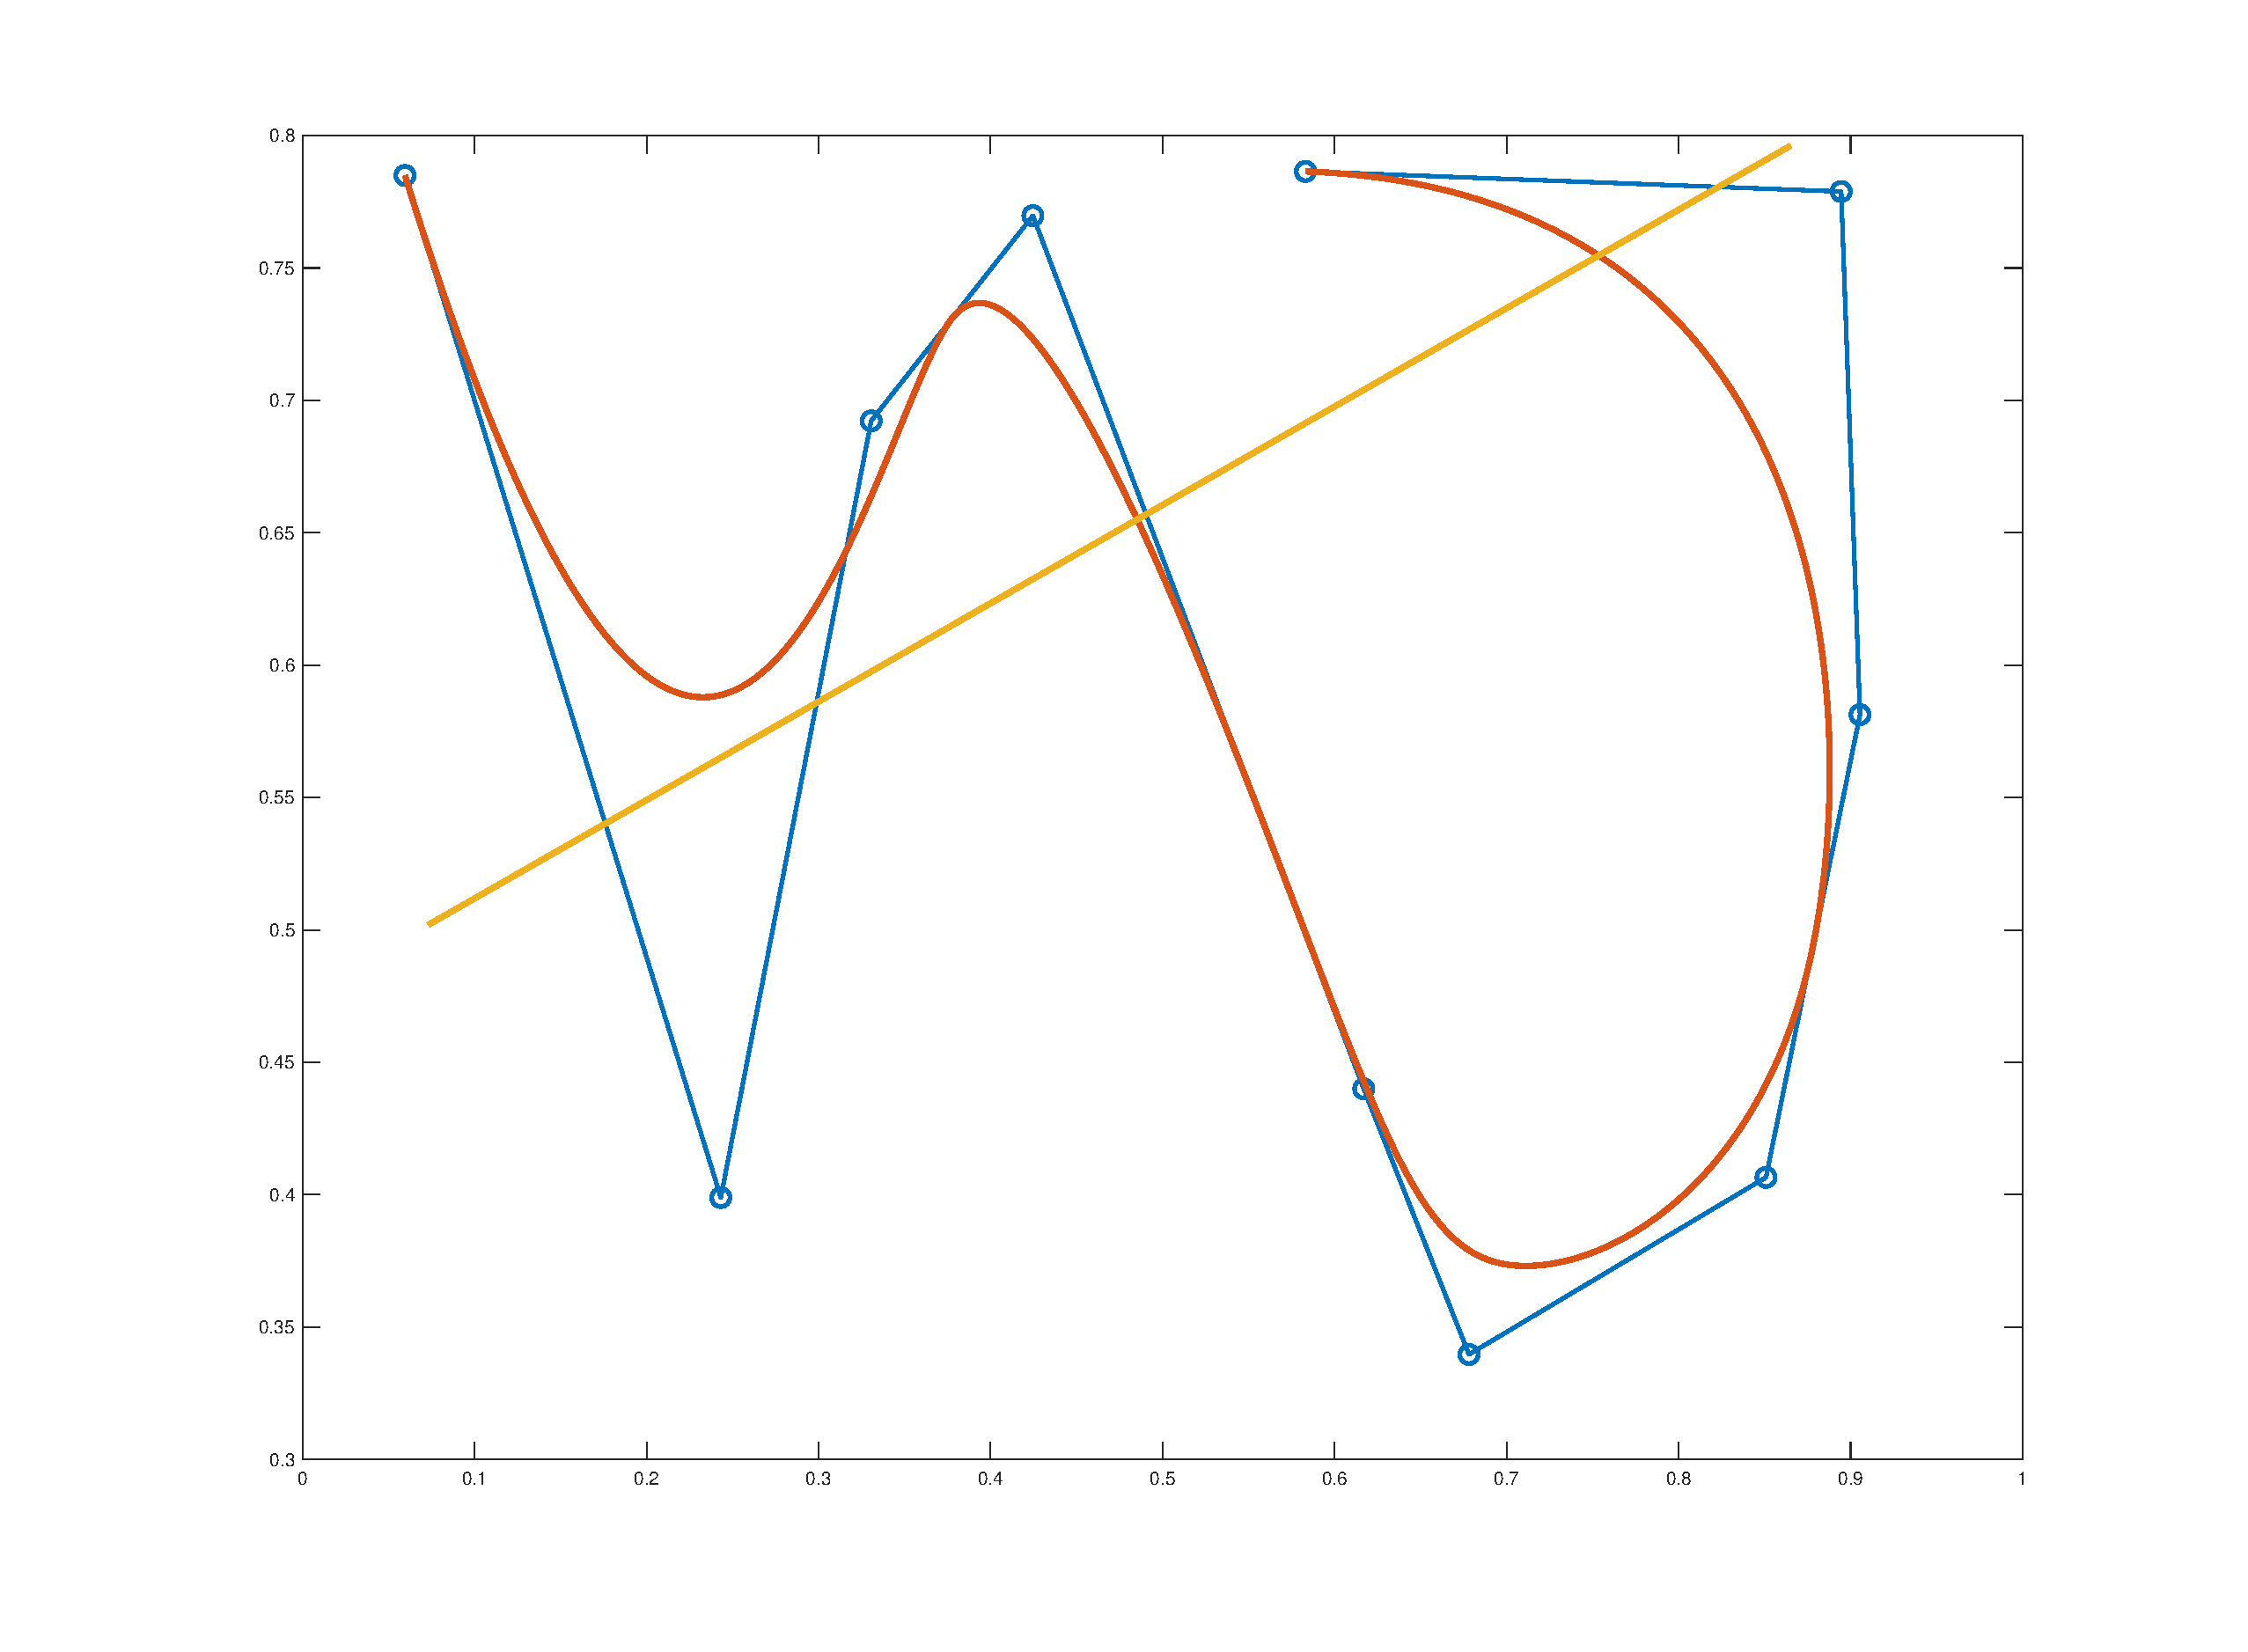
\includegraphics[width=\textwidth]{figure/intersection5.eps}
    \caption{Poligono: $4$, Curva: $2$}
    \label{fig:intersection5}
  \end{subfigure}
  \caption{Proprietà di Variation Diminishing}\label{fig:intersection}
\end{figure}

\subsection{Curve Chiuse}
Grazie ai nodi ausiliari ciclici è possibile usare la base delle B-Spline per generare
curve chiuse. In Codice~\ref{code:closed_curve} è possibile vedere un esempio di implementazione di una curva chiusa di 
ordine $k = 4$.
Per ottenere una curva con questa proprietà è necessario generare una partizione nodale estesa in questo modo:
$$\Delta^* = \left[ \underbrace{\frac{-k}{m-1}}_{Inizio} : \underbrace{\frac{1}{m-1}}_{Passo} : \underbrace{\frac{k+m-1}{m-1}}_{Fine} \right]$$
con $k$ ordine della spline e $m$ numero di vertici di controllo della curva.
Successivamente è anche necessario estendere il poligono di controllo ripetendo i primi $k-1$ vertici.
\lstinputlisting[label=code:closed_curve, firstline=2, language=Matlab, caption = Curva chiusa]{code/b_spline_curve.m}
\begin{figure}[]
  \centering
  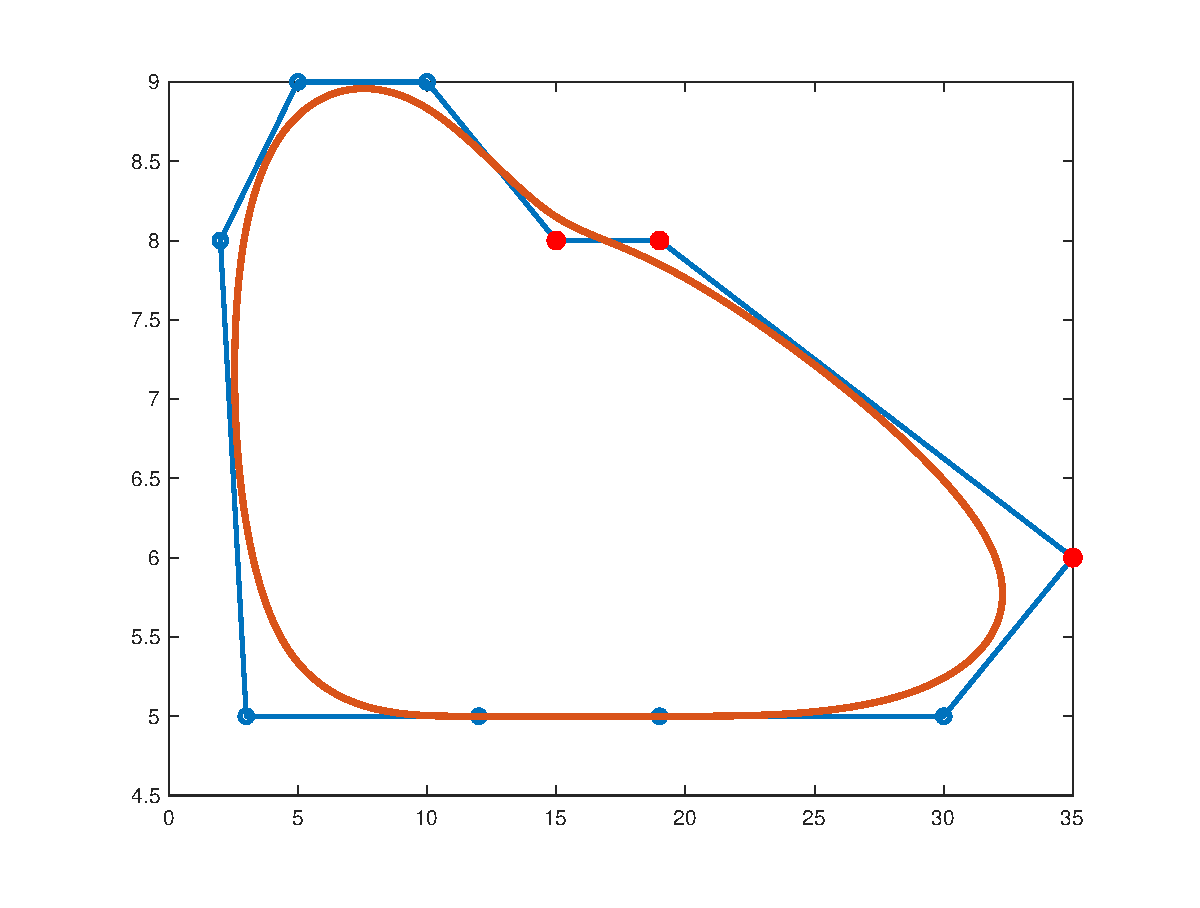
\includegraphics[width=0.75\textwidth]{figure/closed_curve.eps}
  \caption{Curva chiusa (in rosso i vertici ripetuti)}
  \label{fig:closed_curve}
\end{figure} 
In Figura~\ref{fig:closed_curve} è possibile vedere il risultato del Codice~\ref{code:closed_curve}, i vertici di controllo rossi sono 
quelli ripetuti.
TODO: FARE QUALCOSA CON LA CONTINUITÀ

\section{Superfici \textit{Tensor-Product} di Bézier}
Una superficie \textit{Tensor-Product} di Bézier si definisce a partire dalla base di Bézier e da $(n+1)\cdot(m+1)$ vertici di controllo, i 
quali a loro volta formano un poligono di controllo. 
\begin{mydef}
  Una superficie \textit{Tensor-Product} di Bézier è data da:
  $$\mathbf{X}(u, v) = \sum_{i = 0}^{n} \sum_{j = 0}^{m} \mathbf{b}_{i, j} B^{n}_{i}(u)B_{j}^{m}(v) $$
  dove:
  \begin{itemize}
    \item $B^{n}_{i}$ e $B^{m}_{j}$ sono i polinomi di Bernstein rispettivamente di 
    grado $n$ e $m$ e indice $i$ e $j$.
    \item $\mathbf{b}_{i,j}$ sono gli  $(n+1)\cdot(m+1)$ vertici di controllo.
  \end{itemize}
\end{mydef}
Di seguito, in Codice~\ref{code:bezier_basis} un'implementazione della base
per le superfici di Bézier realizzata con l'uso della funzione \texttt{spcol}.
\lstinputlisting[label=code:bezier_basis, firstline=2, language=Matlab, caption = Base delle superfici di Bézier]{code/bezier_surface_basis.m}
\lstinputlisting[label=code:bezier_surface, firstline=2, lastline = 19, language=Matlab, caption = Disegno di una superficie di Bézier]{code/bezier_surface.m}
\begin{figure}[]
  \centering
  \begin{subfigure}[b]{0.3\textwidth}
    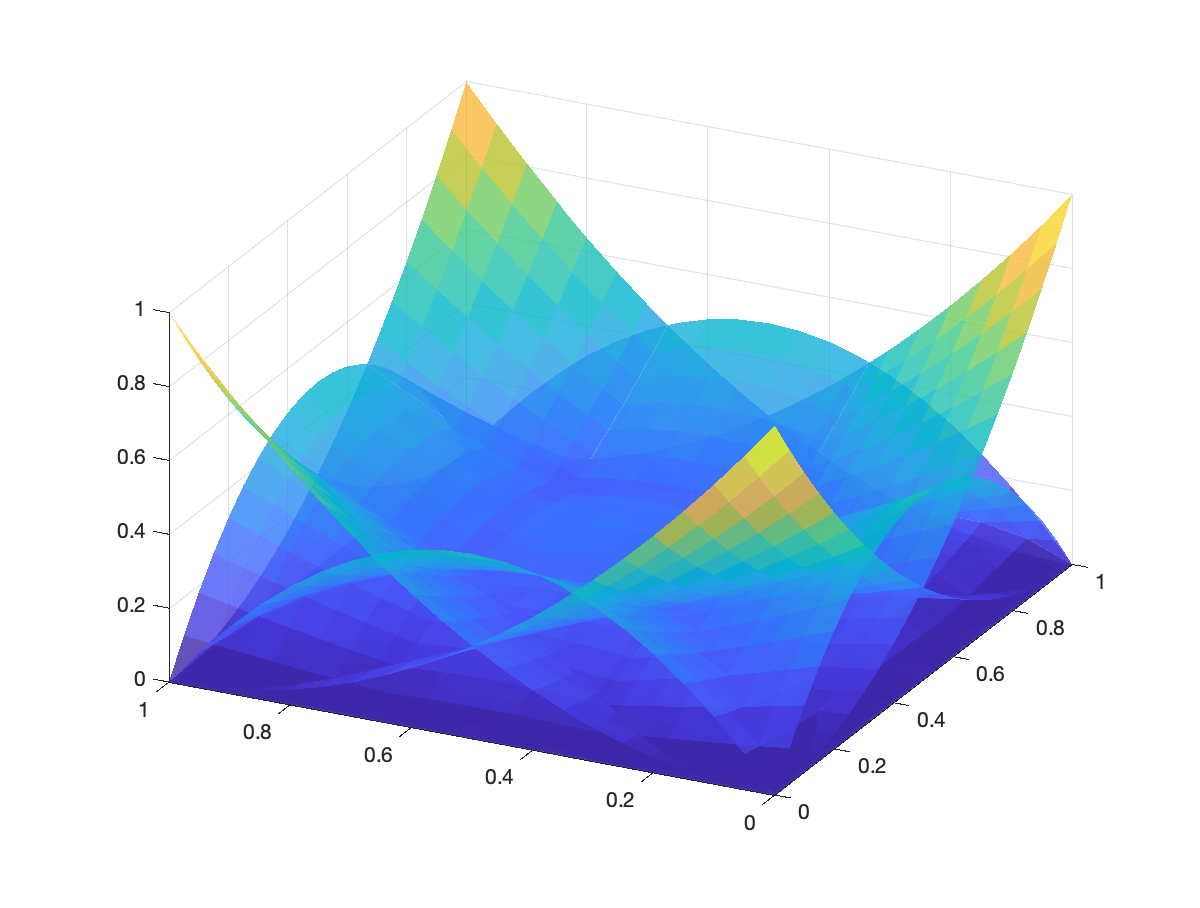
\includegraphics[width=\textwidth]{figure/bezier_surface_basis33_1.eps}
    \caption{$k_u$: $3$, $k_v$: $3$}
    \label{fig:bezier_surface_basis33_1}
  \end{subfigure}
  \begin{subfigure}[b]{0.3\textwidth}
      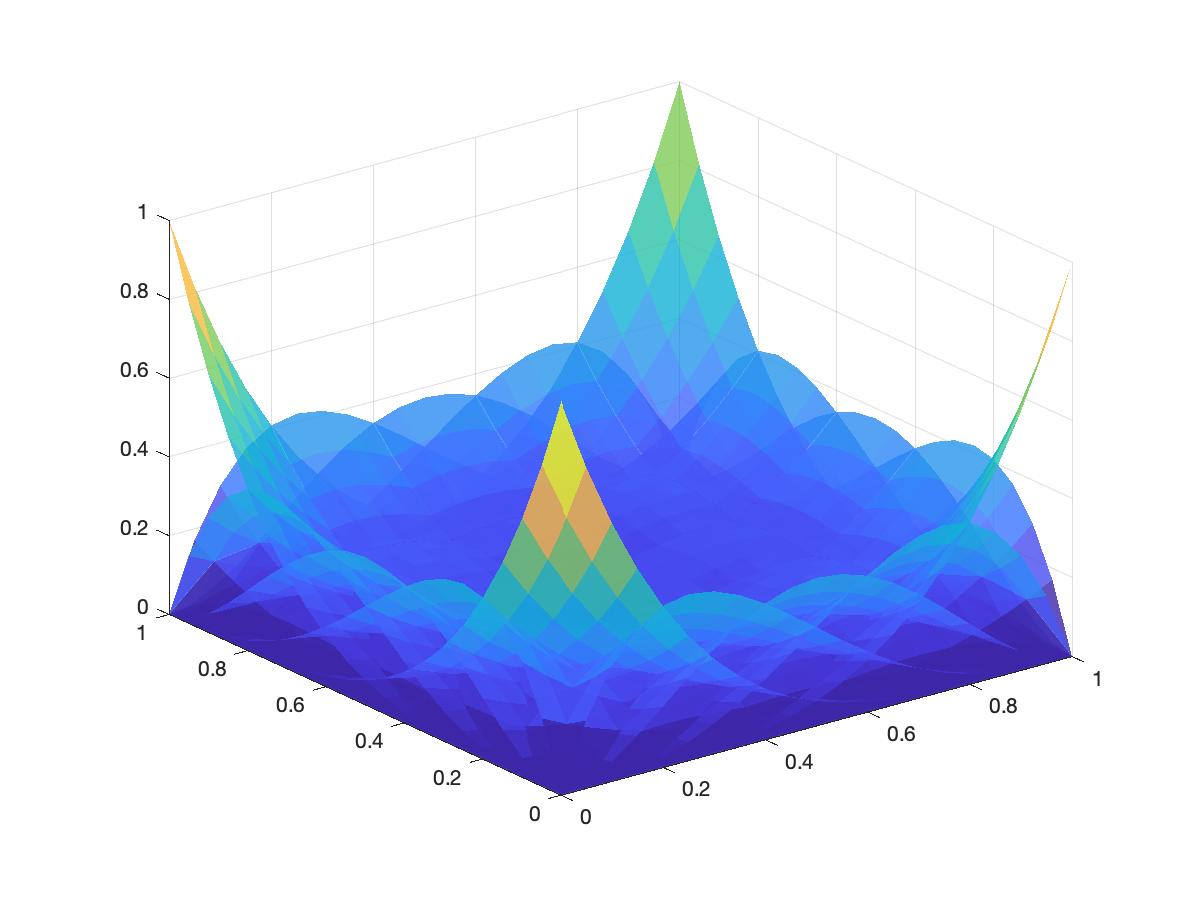
\includegraphics[width=\textwidth]{figure/bezier_surface_basis55_1.eps}
      \caption{$k_u$: $5$, $k_v$: $5$}
      \label{fig:bezier_surface_basis55_1}
  \end{subfigure}
  \begin{subfigure}[b]{0.3\textwidth}
      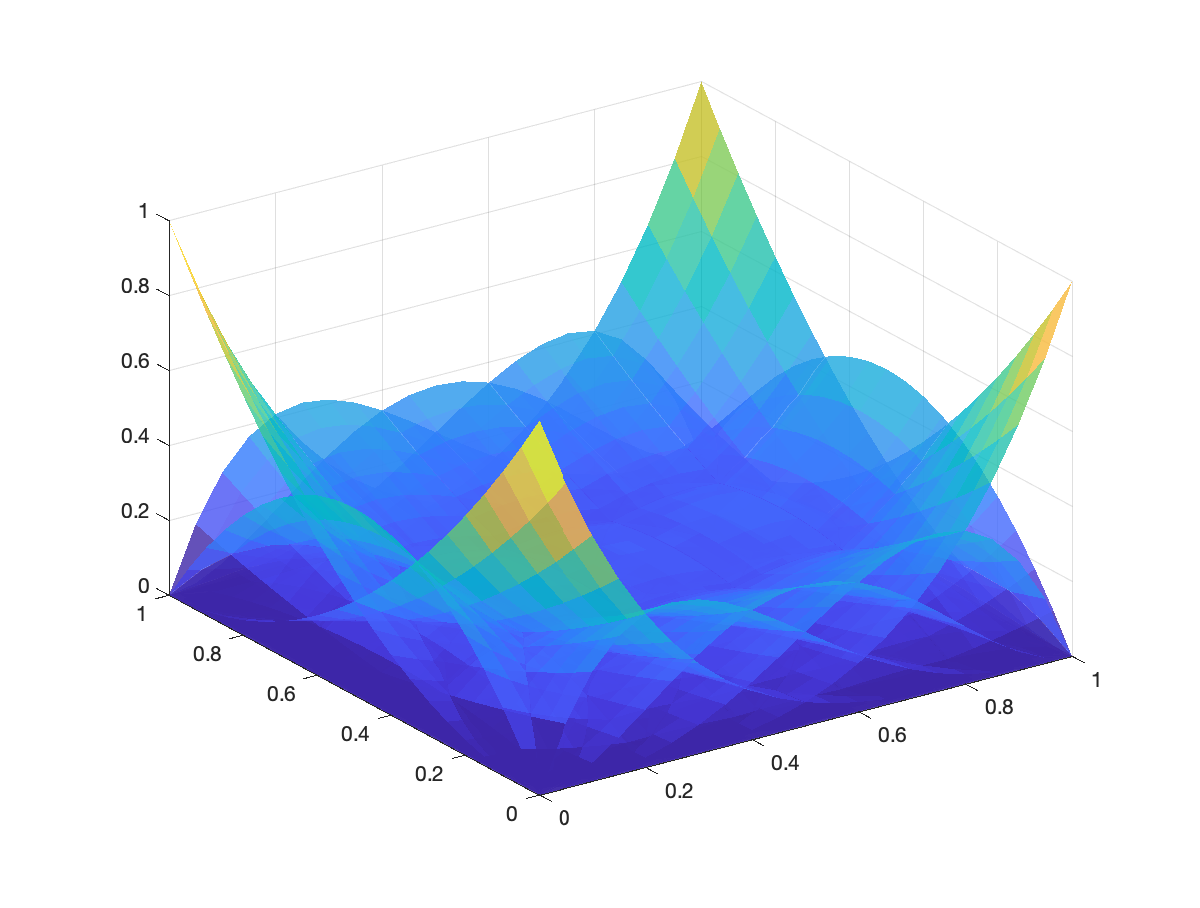
\includegraphics[width=\textwidth]{figure/bezier_surface_basis35_1.eps}
      \caption{$k_u$: $3$, $k_v$: $5$}
      \label{fig:bezier_surface_basis35_1}
  \end{subfigure}
  \caption{Base di Bézier}\label{fig:bezier_basis}
\end{figure}
\begin{figure}[]
  \centering
  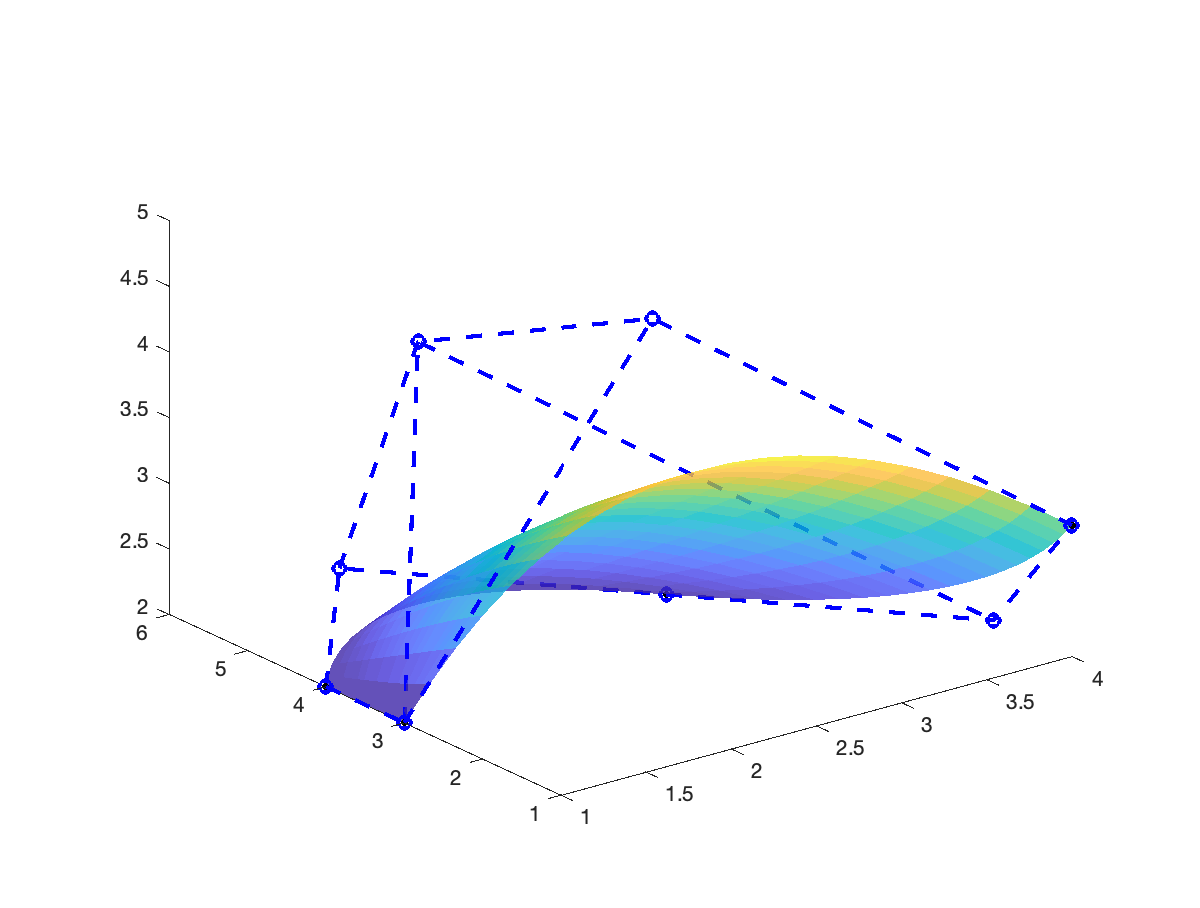
\includegraphics[width=0.75\textwidth]{figure/bezier_surface1.eps}
  \caption{Superficie di Bézier generata da Codice~\ref{code:bezier_surface}}
  \label{fig:bezier_sup_code}
\end{figure} 
\subsection{Proprietà delle superfici di Bézier}
Come per le curve, le superfici di Bèzier godono di alcune proprietà:
\begin{itemize}
  \item Invarianza per trasformazioni affini: applicare una trasformazione affine sui punti di controllo o sulla superfice è indifferente, il risultato sarà uguale.

  \item Convex Hull: DA FARE
  \item Curve di bordo: le quattro curve di bordo della superficie di Bézier sono date da
  $$\mathbf{X}(0,v) = \sum_{j=0}^{m} \mathbf{b}_{0,j}B_{j}^{m}(v) \quad \mathbf{X}(1,v) = \sum_{j=0}^{m} \mathbf{b}_{m,j}B_{j}^{m}(v)$$
  $$\mathbf{X}(u, 0) = \sum_{i=0}^{n} \mathbf{b}_{i,0}B_{i}^{n}(u) \quad \mathbf{X}(u,1) = \sum_{i=0}^{n} \mathbf{b}_{i, m}B_{i}^{n}(u)$$
\end{itemize}
  \paragraph{Invarianza per trasformazioni affini}
  Come detto in precedenza questa proprietà dice che se applicata una trasformazione affine sui punti di controllo o sulla superfice è indifferente. 
  Questo proprietà risulta molto utile nella situazione in cui si deve applicare una determinata trasformazione ad una superficie. Il modo 
  più efficiente per realizzare ciò è applicare la trasformazione ai punti di controllo e successivamente ridisegnare la superfice.
  In Codice~\ref{code:bezier_surf_trans} è possibile vedere l'esempio di un disegno di una superficie e successiva trasformazione,
  sia sui punti di controllo che sulla superficie stessa.
  \lstinputlisting[label=code:bezier_surf_trans, firstline=2, lastline = 46, language=Matlab, caption = Base delle superfici di Bézier]{code/bezier_surface.m}
  In questo caso per mostrare che le due superfici trasformate sono uguali è stata usata la funzione \texttt{isequal}, che restituisce \texttt{1} se e solo se 
  le due matrici in input sono uguali. Il plot in output del Codice~\ref{code:bezier_surf_trans} è mostrato in Figura~\ref{fig:bezier_surf_trans}.
  \begin{figure}[]
    \centering
    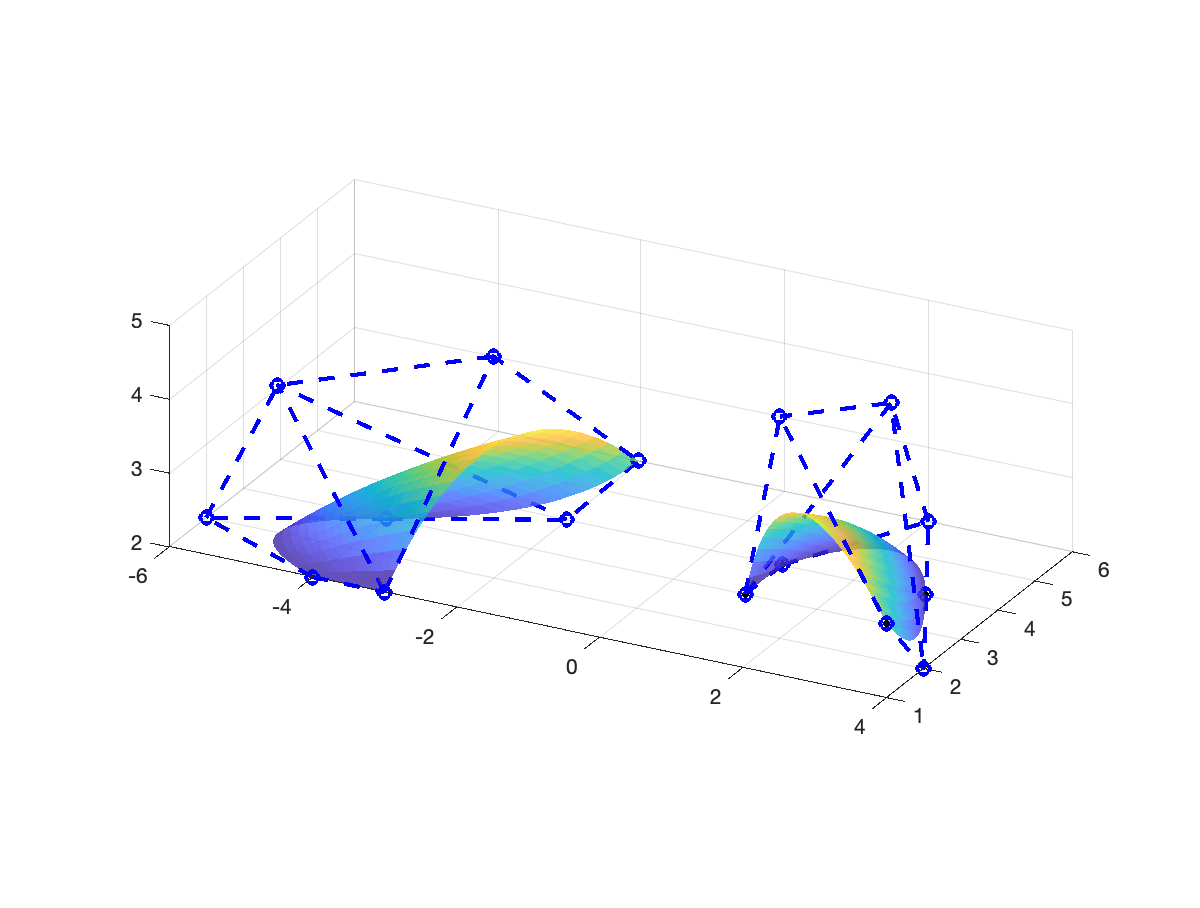
\includegraphics[width=0.75\textwidth]{figure/bezier_surf_trans.eps}
    \caption{Trasformazione affine su una superficie di Bézier}
    \label{fig:bezier_surf_trans}
  \end{figure} 
  \paragraph{Convex Hull} TODO: CODICE, FIGURE, SCRIVERE
  \paragraph{Curve di bordo} I bordi di una superfice di Bézier possono essere visti a loro
  volta come quattro curve di Bézier:
  $$\mathbf{X}(0,v) = \sum_{j=0}^{m} \mathbf{b}_{0,j}B_{j}^{m}(v) \quad \mathbf{X}(1,v) = \sum_{j=0}^{m} \mathbf{b}_{m,j}B_{j}^{m}(v)$$
  $$\mathbf{X}(u, 0) = \sum_{i=0}^{n} \mathbf{b}_{i,0}B_{i}^{n}(u) \quad \mathbf{X}(u,1) = \sum_{i=0}^{n} \mathbf{b}_{i, m}B_{i}^{n}(u)$$
  In Codice~\ref{code:bezier_border_curve} è possibile vedere il calcolo, tramite l'algoritmo di \textit{De Casteljau}, di una delle quattro curve di bordo, 
  mentre in Figura~\ref{fig:bezier_border_curve} è possibile vedere 
  il plot dei bordi di una superficie di Bézier.
\begin{figure}[]
  \centering
  \begin{subfigure}[b]{0.3\textwidth}
    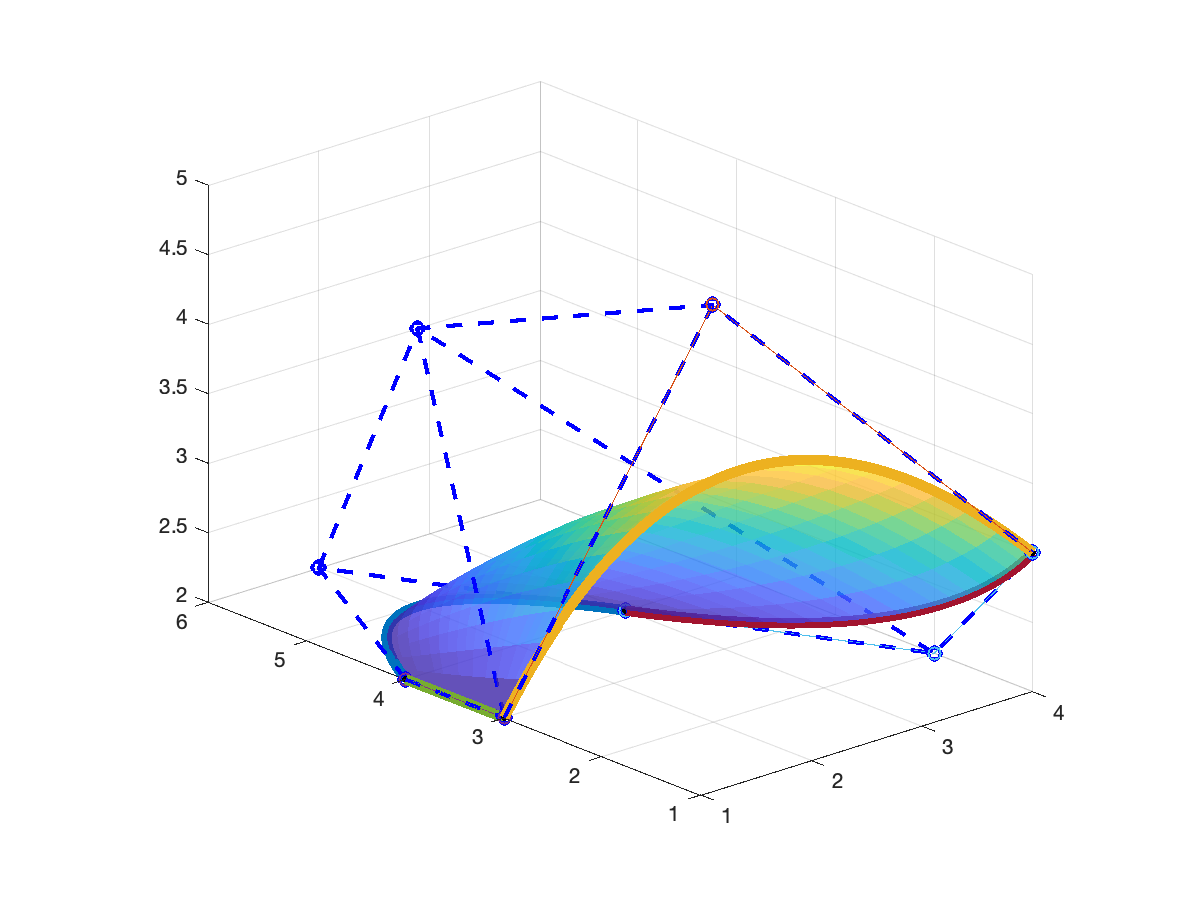
\includegraphics[width=\textwidth]{figure/border_curve.eps}
    \label{fig:border_curve}
  \end{subfigure}
  \begin{subfigure}[b]{0.3\textwidth}
      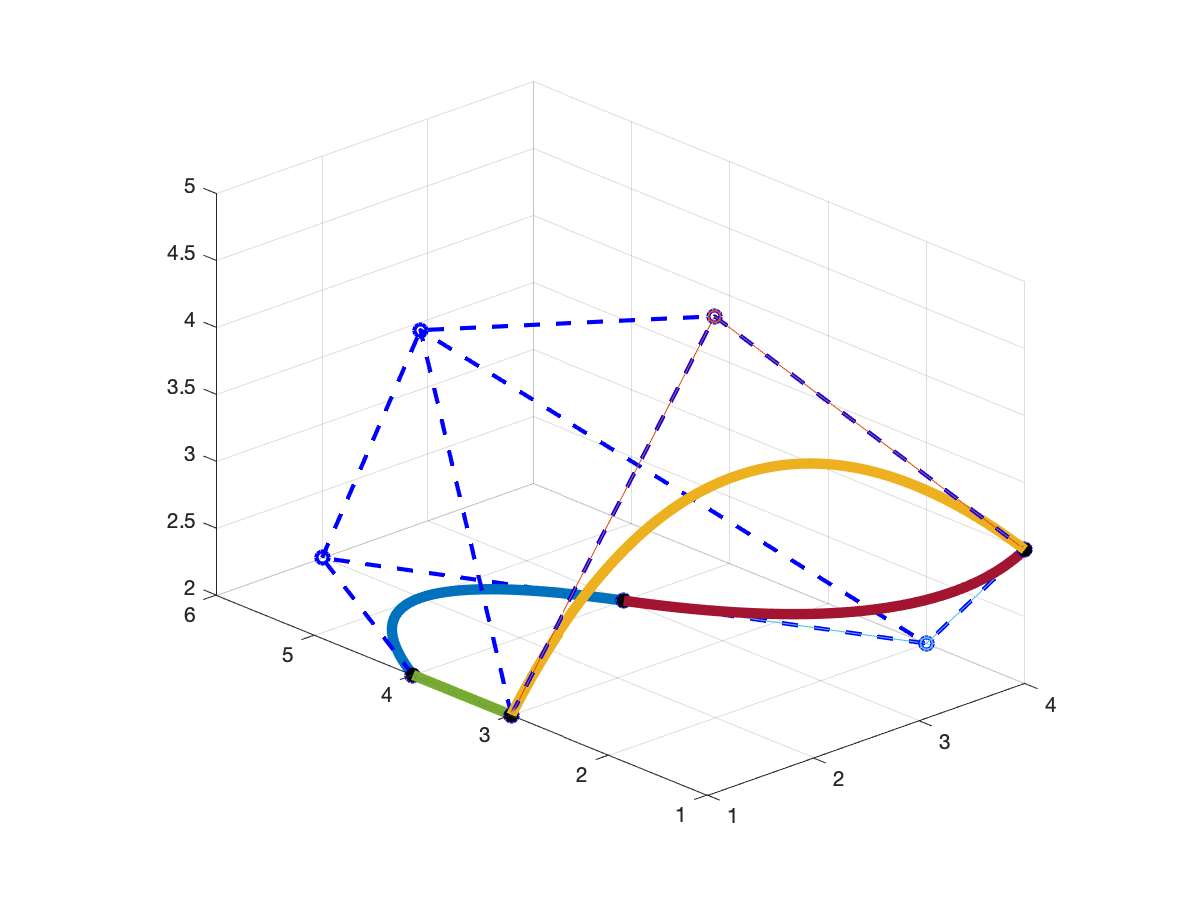
\includegraphics[width=\textwidth]{figure/border_curve_no_surf.eps}
      \label{fig:border_curve_no_surf}
  \end{subfigure}
  \begin{subfigure}[b]{0.3\textwidth}
      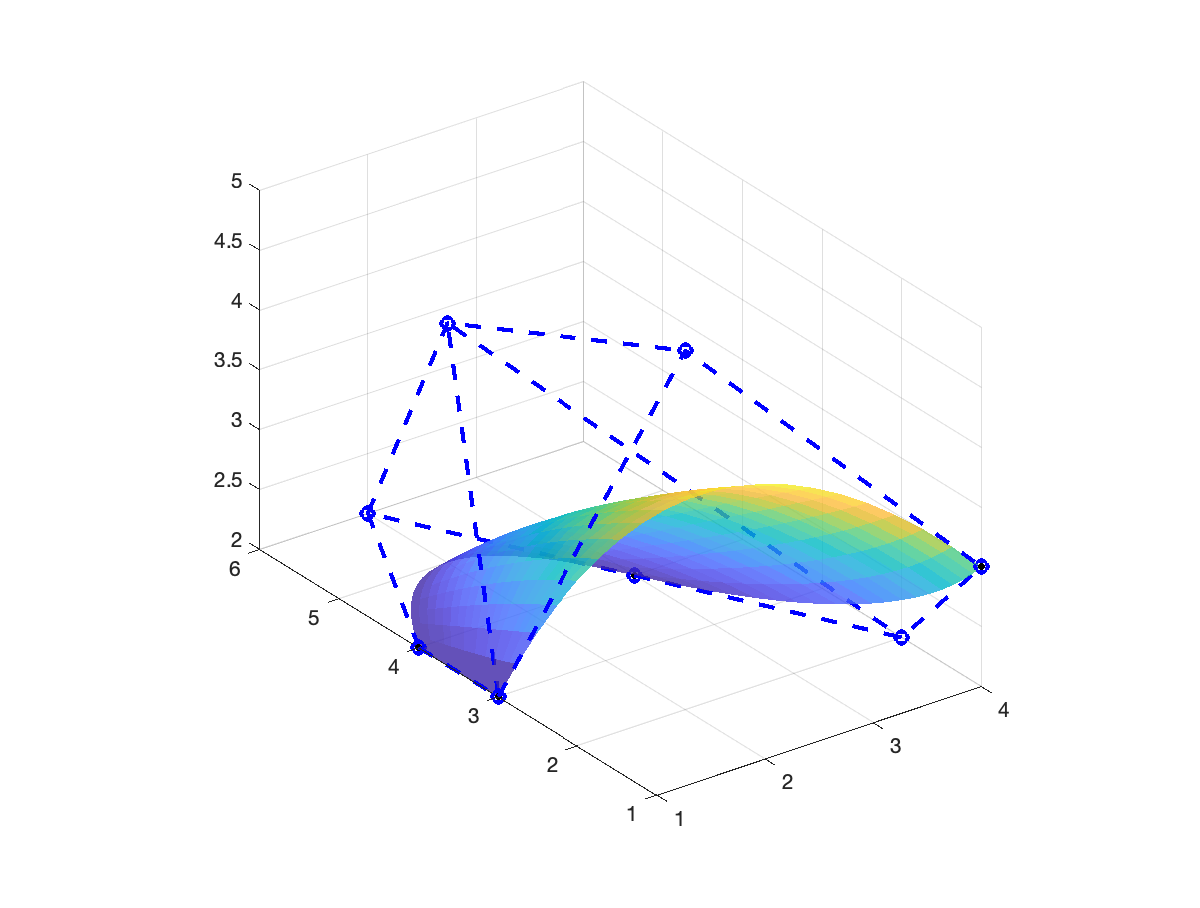
\includegraphics[width=\textwidth]{figure/surf_no_bord.eps}
      \label{fig:surf_no_bord}
  \end{subfigure}
  \caption{Curve di bordo}\label{fig:bezier_border_curve}
\end{figure}
\lstinputlisting[label=code:bezier_border_curve, firstline=76, lastline = 84, language=Matlab, caption = Base delle superfici di Bézier]{code/bezier_surface.m}
\subsection{Algoritmo di De Casteljau}
TODO: FINIRE CODICE, FIGURE, SCRIVERE


\end{document}
